\documentclass[ a4paper,
  abstract=false,
  twoside,
  listof=totoc,
  numbers=noenddot,
  bibliography=totoc,
  headsepline,
  appendixprefix,
final]{scrreprt}
\KOMAoptions{titlepage=firstiscover,twoside,listof=totoc, BCOR=1.5cm, DIV=12}

\usepackage{subcaption}
\usepackage[english]{babel}
\usepackage[utf8]{inputenc}
\usepackage[T1]{fontenc}
\usepackage[hidelinks=true]{hyperref}
\usepackage{clrscode}
\usepackage[dvipsnames]{xcolor}
\usepackage[pdftex]{graphicx}
\usepackage[lsb=1]{bytefield}
\usepackage[justification=centering]{caption}
\usepackage[acronym,nomain,toc]{glossaries}
\usepackage{mathtools}
\usepackage{amssymb}
\usepackage{todonotes}
\usepackage{listings}
\usepackage{multirow}
\usepackage{setspace}
\usepackage{geometry}
\usepackage{tabularx} % book-quality tables
\usepackage{booktabs} % book-quality tables
\usepackage{float}
\usepackage{tikz}
\usepackage[final]{microtype}
\usepackage[nottoc]{tocbibind}
\usepackage{csquotes}% Recommended
\usepackage{pdfpages}
\usepackage[backend=biber,style=alphabetic,alldates=long]{biblatex}
\usepackage{chngcntr}

\usetikzlibrary{arrows.meta}
\addbibresource{references.bib}

\input{style.tex}

% Colors
\definecolor{pastelgreen}{RGB}{190, 219, 57}
\definecolor{pastelred}{RGB}{255, 117, 97}
\definecolor{pastelorange}{RGB}{255, 210, 87}

\pgfdeclarelayer{bg}    % declare background layer
\pgfsetlayers{bg,main}  % set the order of the layers (main is the standard layer)

\renewcommand{\arraystretch}{1.2} % Nice tables

\usetikzlibrary{matrix,calc,shapes,positioning}
\lstset{
    showstringspaces=false,
    basicstyle=\ttfamily,
    keywordstyle=\color{blue},
    commentstyle=\color[gray]{0.6},
    stringstyle=\color[RGB]{255,150,75}
}
\renewcommand{\lstlistingname}{Source Code}
\newcommand{\inlinecode}[2]{\colorbox{white}{\lstinline[language=#1]$#2$}}
\newcommand{\documenttitle}{Enhancements for MACsec providing transparent Layer-2 encryption}

\newcommand{\colorbitbox}[3]{%
\rlap{\bitbox{#2}{\color{#1}\rule{\width}{\height}}}%
\bitbox{#2}{#3}}

\newcommand{\colorbitboxProp}[4]{%
\rlap{\bitbox[#4]{#2}{\color{#1}\rule{\width}{\height}}}%
\bitbox[#4]{#2}{#3}}

\newcommand{\colorwordbox}[3]{%
\rlap{\wordbox{#2}{\color{#1}\rule{\width}{\height}}}%
\wordbox{#2}{#3}}

\newcommand{\colorwordboxProp}[4]{%
\rlap{\wordbox[#4]{#2}{\color{#1}\rule{\width}{\height}}}%
\wordbox[#4]{#2}{#3}}

\graphicspath{{./figures/}}

\glsdisablehyper

\newacronymstyle{long-em-short}%
  {% use the same display as "long-short"
  \GlsUseAcrEntryDispStyle{long-short}%
  }%
  {% use the same definitions as "long-short"
  \GlsUseAcrStyleDefs{long-short}%
  % Minor modifications:
  \renewcommand*{\genacrfullformat}[2]{%
    \firstacronymfont{\emph{\glsentrylong{##1}} (\glsentryshort{##1})}%
  }
  \renewcommand*{\genplacrfullformat}[2]{%
    \firstacronymfont{\emph{\glsentrylongpl{##1}} (\glsentryshortpl{##1})}%
  }
}

\setacronymstyle{long-em-short}
%!TEX root=thesis.tex
\newacronym{ISO}{ISO}{International Standards Organisation}
\newacronym{MAC}{MAC}{Medium Access Control}


\newacronym{MTU}{MTU}{Maximum Transmission Unit}
\newacronym{PMTUD}{PMTUD}{Path MTU Discovery}

\newacronym{OSI}{OSI}{Open Systems Interconnection}
\newacronym{MACsec}{MACsec}{Medium Access Control Security}
\newacronym{ICV}{ICV}{Integrity Check Value}
\newacronym{MPDU}{MPDU}{MACsec Protocol Data Unit}
\newacronym{SecTAG}{SecTAG}{Security TAG}
\newacronym{AN}{AN}{Association Number}
% Nummer, die mit Secure Channel Identifier konkateniert wird, um eine Secure Association zu identifizieren

\newacronym[longplural={MAC Security Entities}]{SecY}{SecY}{MAC Security Entity}
%Entität, die MACSec durchführt
\newacronym[longplural={MAC Security Key Agreement Entities}]{KaY}{KaY}{MAC Security Key Agreement Entity}


\newacronym{MSDU}{MSDU}{MAC Service Data Unit}
\newacronym{FIFO}{FIFO}{First in, First out}

\newacronym{PN}{PN}{Packet Number}
\newacronym{Qdisc}{Qdisc}{Queueing Discipline}

\newacronym{PDU}{PDU}{Protocol Data Unit}
%Das, was eine Schicht erzeugt

\newacronym{SA}{SA}{Secure Association}
% Security Relationship that provides security guarantees for frames transmitted from one member of the CA to others

\newacronym{SAI}{SAI}{Secure Association Identifier}
% Identifier für SA, besteht aus SCI konkateniert mit AN

\newacronym{SAK}{SAK}{Secure Association Key}
%Secret Key, der von SA genutzt wird

\newacronym{SL}{SL}{Short Length}
\newacronym{SC}{SC}{Secure Channel}
%Security Relationship used to provide security guarantees for frames transmitted from one member of the CA to others, supported by a sequence of SAs allowing periodic use of fresh keys

\newacronym{SDU}{SDU}{Service Data Unit}

\newacronym{IV}{IV}{Initialization Vector}
\newacronym{IP}{IP}{Internet Protocol}
\newacronym{MF}{MF}{More Fragments}
\newacronym{WLAN}{WLAN}{Wireless LAN}

\newacronym{LTE}{LTE}{Long Term Evolution}
\newacronym{RLC}{RLC}{Radio Link Control}
\newacronym{TM}{TM}{Transparent Mode}
\newacronym{AM}{AM}{Acknowledged Mode}
\newacronym{UM}{UM}{Unacknowledged Mode}
\newacronym{UMD}{UMD}{\acrlong{UM} Data}

\newacronym{SN}{SN}{Sequence Number}
\newacronym{E}{E}{Extension}
\newacronym{LI}{LI}{Length Indicator}
\newacronym{FI}{FI}{Framing Info}

\newacronym{SCI}{SCI}{Secure Channel Identifier}
%Globally Unique Identifier für Secret Channels, bestehend aus MAC und Port Identifier
\newacronym{TCI}{TCI}{TAG Control Information}
\newacronym{TCP}{TCP}{Transmission Control Protocol}

\newacronym{CA}{CA}{Secure Connectivity Association}
\newacronym{IEEE}{IEEE}{Institute of Electrical and Electronics Engineers}
\newacronym{LAN}{LAN}{Local Area Network}

\newacronym{SEGL}{SEGL}{Segment Length}
\newacronym{RTT}{RTT}{Round-trip time}
\newacronym{ICMP}{ICMP}{Internet Control Message Protocol}

\makeglossaries
\date{March 26,  2018}
\newcommand{\printdate}{\@date}

\begin{document}
\pagenumbering{Roman}

  \begin{singlespace}

    \subject{{\LARGE Bachelor's Thesis}}

    \title{\documenttitle}

    \author{Jan Sönke Huster}

    \publishers{TU Dresden\\
    Faculty of Computer Science\\
    Institute of Systems Architecture\\
    Chair of Privacy and Data Security\\
    \begin{minipage}{\textwidth}%\\
      \vskip 6cm
       {\normalsize }
       \begin{tabular}{ll}
        Professor: &
        Prof. Dr. Thorsten Strufe\tabularnewline
        Supervisors: &
        Dr.-Ing. Stefan Köpsell\tabularnewline
        & Dipl. Inf. Tim Lackorzynski \tabularnewline
      \end{tabular}{\normalsize }
    \end{minipage}}

    \maketitle
  \end{singlespace}
  \cleardoublepage

  \includepdf{./Aufgabenstellung.pdf}
  \cleardoublepage

  \section*{\vfill{} \thispagestyle{empty}
  Erklärung / Declaration}

  Hiermit erkläre ich, dass ich diese Arbeit selbstständig erstellt und keine anderen als die angegebenen Hilfsmittel benutzt habe.

  \bigskip{}
  \noindent I hereby declare that I completed this work on my own and have not used any resources other than those noted.
  \bigskip{}

  \noindent Dresden, March 26,  2018
  \vspace{2.5cm}

  \noindent Jan Sönke Huster \cleardoublepage{}

  \microtypesetup{protrusion=false} % disables protrusion locally in the document
  \tableofcontents
  \listoffigures
  \listoftables
  \cleardoublepage
  \glsresetall
  \microtypesetup{protrusion=true} % enables protrusion locally in the document

  \pagenumbering{arabic}
  %!TEX root=../thesis.tex
\chapter{Introduction}
\label{ch:intro}
As Industry 4.0 becomes more popular, networking in factories has gotten more important.
However, current factories are insecure as a study of the german Federal Ministry of Economic Affairs and Energy regarding IT security in Industry 4.0 shows~\cite{studiebmwi}.
The FastVPN project\footnote{\url{https://en.fast-zwanzig20.de/industrie/fast-vpn-2/}} adresses this problem space.

It provides transparent network bridges---FastVPN boxes---, which are deployed between industry machines and the factory network.
Thus the network communication is encapsulated, furthermore, network security inbetween the FastVPN boxes is improved.
This environment is displayed in figure~\ref{fig:environment}.

\begin{figure}[!h]
  \centering
  \def\svgwidth{0.8\columnwidth}
  \input{./figures/environment.pdf_tex}
  \caption[FastVPN Setup Example]{Insecure network communication is protected by FastVPN boxes. The is done by applying MACsec. The \acrlong{MTU} between the boxes is smaller than the one between client and box.}
  \label{fig:environment}
\end{figure}

A protocol used by the FastVPN box to improve network security is \gls{MACsec}, a standard of the \gls{IEEE}.
\gls{MACsec} provides confidentiality and integrity on the data link layer.
It encrypts network communication and protects against unauthorized modification by appending a message authentication code.
The downside of \gls{MACsec} is the reduction of the maximum packet size---the \gls{MTU}--- because additional information are added to each frame which is tunneled through the FastVPN box.

If machines cannot discover that the \gls{MTU} is decreased on the path, the packets are oversized at one point.
The standard behavior is to drop these oversized packets.
As a result, machines without this discovery mechanism are not able to communicate through the FastVPN box.

A solution to this problem can be the use of jumbo frames, which allow higher \gls{MTU} sizes than the standard of 1500 bytes.
By enabling jumbo frames between the FastVPN boxes, the \gls{MTU} can be increased so that the overhead introduced by \gls{MACsec} is equalized.
But to enable jumbo frames modern network hardware between the FastVPN boxes is required.

The aim of the FastVPN project is the deployment in factories.
Machines as well as network hardware in factories often have a long life span, so the FastVPN project cannot assume that the configuration of jumbo frames is feasible.
Furthermore, it is not assumed that the machines are discovering the decreased \gls{MTU}.

Therefore, it requires a solution to use \gls{MACsec} without a reduction of the \gls{MTU} and the configuration of jumbo frames.
The aim of this thesis is to develop a transparent fragmentation solution in combination with \gls{MACsec} to solve this problem.
As the reduction of the \gls{MTU} is comparatively small to the frame size, a simple split produces one full and one very small frame.
Hence, possible optimizations are examined.

This thesis begins with an introduction into computer networks, security and \gls{MACsec}.
Moreover, protocols which support fragmentation and possible optimizations are examined.
Afterwards, several approaches to implement fragmentation when using \gls{MACsec} are proposed and discussed.
The most promising solution is then specified in detail and implemented for the use with linux.
Finally, the implementation of the proposed fragmentation scheme is evaluated regarding security and performance.
Therefore, it is compared with the solution of using jumbo frames.

  %!TEX root=../thesis.tex
\chapter{Related Work}
%!TEX root=../thesis.tex
\section{Computer Networks}
The following sections give a short introduction into computer network theory and provide an explanation to the terms used in this thesis.
If not otherwise noticed, the information of this section is taken from~\cite{tanenbaum2011networks}.

\begin{figure}
  \centering
  \def\svgwidth{\columnwidth}
  \input{./figures/osi.pdf_tex}
  \caption[\acrshort{OSI} Model]{The first 4 layers of the \gls{OSI} model. Host 1 sends a message to Host 2, one layer 3 and one layer 2 switch are involved.}
  \label{fig:osi}
\end{figure}

\paragraph{OSI model}
The \gls{OSI} model is a reference model for computer network architecture proposed by the \gls{ISO} in~\cite{isoosi1994}.

It defines seven layers which are stacked on top of each other like displayed in figure~\ref{fig:osi}.
Every layer is just able to communicate with its neighbouring layers and performs a well defined function, such as layer 1 (physical layer) transmits bytes on a medium.

When an application transmits data to another host the data is traveling the path from the top layer (application layer) to the bottom layer, which is the physical layer.
Each layer on this path performs its function on the data.
The recipient receives the data and each layer processes it, from the lowest back to the top layer.
Also the devices in between the network have a layered architecture and are processing the transmitted data in their layers.
Those devices in the network which determine the path of transmitted data (``routing'') usually have three or two layers as shown in figure~\ref{fig:osi}.

Data received by a layer from the layer above is named \gls{SDU}.
The processed data, which a layer is passing down to the next layer, is called \gls{PDU}.
\glspl{PDU} have different names, depending on the layer.
On layer 2 they are named ``frames'' and on layer 3 they are named ``packets''.
 A generic term is ``datagram''~\cite{RFC1594}.

Relevant layers for this thesis are the network layer (layer 3) and the data link layer (layer 2).

\paragraph{Layer 3}
\label{par:layer-3}
The network layer is determining the route of a packet and makes communication with other networks possible.
Furthermore, it adapts the \gls{SDU} to the \gls{MTU}, which is the maximum size a data packet can have.
Therefore, it breaks the \gls{SDU} in several fragments and sends them as single packets.
The receiving network layer is able to reassemble the fragments and passes them as a whole to the overlaying layer.
This is possible because each layer is able to put more information into each \gls{SDU} by transforming it or prepending and appending data.
Usually a layer prepends a header with information on the \gls{SDU} on transmission.
When it receives a \gls{PDU} to pass it to an upper layer, the information is processed and stripped.
One of the usual protocols that work on layer 3 is the \gls{IP}.
The fragmentation process of \gls{IP} is described in section~\ref{sec:ip-fragmentation}.

\paragraph{Layer 2}
The data link layer communicates in the same subnetwork and consists of two sublayers.
The Logical Link Control sublayer enables multiplexing.
On shared channels the \gls{MAC} sublayer is checking if the channel is already in use and if a frame can be transmitted.
Furthermore, it passes data to the physical layer.
The \gls{SDU} is put into a frame, source and destination addresses are added, as well as a checksum for error detection.
In a cable-based \gls{LAN} usually Ethernet is used at the data link layer.
A \gls{LAN} is a network which operates in a small area, such as one building.

\begin{figure}
  \centering
  \begin{bytefield}[bitwidth=0.04\columnwidth]{25}
    \bitbox{4}{Preamble} & \bitbox{4}{Destination} & \bitbox{4}{Source} &
    \bitbox{2}{Type} &
    \bitbox{6}{Payload} &
    \bitbox{1}{\tiny P\\a\\d} & \bitbox{4}{Checksum}
  \end{bytefield}
  \caption{Ethernet \acrlong{PDU}}
  \label{fig:ethernet}
\end{figure}

\paragraph{Switched Ethernet}
Ethernet is standardized by the \gls{IEEE} 802.3\footnote{\url{http://www.ieee802.org/3/}} working group.
The terms ``\gls{IEEE} 802.3'' and ``Ethernet'' are interchangeable.
Classical Ethernet used a shared medium to transmit data, which means the physical cable was used by more than one participant at a time.
This evolved to Switched Ethernet, here a dedicated cable per transmission channel is used.

Data is sent in frames and each frame has a preamble (7 bytes), source (6 byte), destination (6 byte) and ethertype (2 byte) prepended as shown in figure~\ref{fig:ethernet}.
The preamble is a constant value to synchronize the clocks of sender and receiver.
Source and destination addresses are 6 bytes long and unique, so every participant can derive if he is the receiver of the frame.
The ethertype field (2 bytes) is used to distinguish different protocols, so the receiver knows what type of data the payload is.
Ethertypes can be requested by anyone at the \gls{IEEE}.
The Ethertype for \gls{MACsec} is 0x88E5.
Furthermore, a checksum (4 bytes) is appended, so the receiver is able to detect errors that happend on transmission.
If an error is detected the frame is dropped, so Ethernet does not guarantee a successful transmission.
An Ethernet frame has to have a minimum size of 64 bytes and a maximum size of 1522 bytes without the preamble, therefore, the payload can usually have a maximum size of 1500 bytes.
If it has less than 46 bytes, padding has to be used.

\paragraph{Switches \& Router}
A switch is a device which has a direct connection to several participants or other switches and forwards received frames to the destination.
A layer 2 switch uses the information in the Ethernet frame header to determine the destination.
As it works on layer 2, it can just forward packets in the same network.
A layer 3 switch---or router---is able to route packets and uses the information of the \gls{IP} to determine the destination.
Therefore, it is able to route between different networks or fragment packets.

\paragraph{MTU}
The \acrfull{MTU} is the maximum size of a data unit to be transmitted.
As prior mentioned, the Ethernet \gls{MTU} is for example 1500 bytes, for \acrlong{WLAN} it is 2272 bytes~\cite{ieeewlan}.
The protocol used in layer 3---which is in practice mostly \gls{IP}---fragments the \glspl{SDU} to match the \gls{MTU}.

The Path \gls{MTU} is the minimum \gls{MTU} on the path a packet travels.
To determine the Path \gls{MTU} a process named \gls{PMTUD} is used, which is specified in \cite{RFC1191}.

\paragraph{Jumbo Frames}
Additionally, there is the possibility of raising the \gls{MTU} up to 9000 bytes while using at least Gigabit Ethernet.
Frames with a size higher than 1500 bytes are called Jumbo Frames.
This is not standardized, but supported by most vendors of network interfaces.

\paragraph{\acrlong{TCP}}
\gls{TCP} is a protocol which resides on layer 4---the transport layer---of the \gls{OSI} model.
It was first specified in RFC~793~\cite{RFC0793}.
It builds a connection over a network and provides a reliable transmission of packets.
To achieve reliability, the receiver sends an acknowledgement for received packets.
If these are not received by the sender after a certain time the packets are resend.

\paragraph{\acrlong{ICMP}}
The \gls{ICMP} is a companion protocol for \gls{IP}.
Its first specification was in~\cite{RFC0792}.
If for example the size of an \gls{IP} packet is bigger than the \gls{MTU}, an \gls{ICMP} message is sent to report this to the sender.
Furthermore, it is used to send ``echo'' messages to check if a machine is reachable which then answers with an ``echo reply'' message.
This can be used to measure the \gls{RTT}, which is the time from sending a packet until receiving the acknowledgement.

%!TEX root=../thesis.tex
\pagebreak
\section{Security}
The following sections introduce the computer security terms, which are needed for this thesis.

\paragraph{Security Goals}
There are three main security goals: confidentiality, integrity and availability~\cite{pfleeger2015security}.
Confidentiality means that information is kept private and just accessable by authorized entities.
Integrity means that unauthorized modification of information is detectable and availability means that a service or data is available and usable~\cite{pfitzmann2012security}.
These goals can be achieved through different techniques, confidentiality for example can be achieved by using encryption.

\paragraph{Symmetric Encryption}
Symmetric encryption describes the class of encryption algorithms, where the same secret is used for encryption and decryption.
The communication partners that want to achieve confidentiality, therefore, they need a shared secret~\cite{pfitzmann2012security}.

\paragraph{Message Authentication Code}
A message authentication code is a symmetric system to check if a message has been manipulated by an unauthorized entity.
Message authentication codes help to achieve integrity.
Authorized entities need a shared secret to create and verify a message authentication code~\cite{pfitzmann2012security}.

\paragraph{Denial-of-Service}
A denial of service attack is an attack targeting the availability of data or a service.
One example for a Denial-of-Service attack is the flooding of a network with unneccessary information to overload it~\cite{pfleeger2015security}.

\paragraph{Replay attack}
Another attack is the replay attack.
Here the attacker delays or repeats valid messages between two parties to gain information~\cite{pfleeger2015security}.

%!TEX root=../thesis.tex
\section{\acrshort{IEEE} 802.1AE \acrshort{MACsec}}
\label{sec:macsec}
The Standard for \acrfull{MACsec} has been published by the \gls{IEEE} in 2006~\cite{macsec}.
\gls{MACsec} is a protocol on layer 2 that provides confidentiality, integrity and data origin authenticity to mitigate network attacks.
Furthermore, it prevents replay attacks.

\subsection{Process}
The entity which is operating \gls{MACsec} is named \gls{SecY}.
For the operation of \gls{MACsec} cryptographic keys are needed because symmetric encryption and message authentication codes are used.
The entity that provides these is the \gls{KaY}.
How the \gls{KaY} works is not specified in the \gls{MACsec} standard but in IEEE 802.1X~\cite{ieee-802-1-x}.
It discovers other \glspl{KaY} that are attached to the same \gls{LAN}, mutually authenticates and authorizes them.
Thereby secure relationships are created, which the \gls{KaY} maintains.
The participants of these secure relationships form one \gls{CA}.
A \gls{SecY} can only be a member of one \gls{CA}.

The \gls{CA} is a group of \glspl{SecY}.
All members of a \gls{CA} use the same cipher suite, which defaults to GCM-AES-128.
With the amendment of 2011 GCM-AES-256 was added~\cite{macsecamendment1}.
The communication of the \gls{CA} members takes place through \glspl{SC}.

A \gls{SC} is a channel from one to many members within a \gls{CA}.
\glspl{SC} support the secure frame transmission using symmetric cryptography.
To distinguish different \glspl{SC} every \gls{SC} has an \gls{SCI}.
A \gls{SC} is supported by successive \glspl{SA}.

Each \gls{SA} uses an individual \gls{SAK}, which is provided by the \gls{KaY}.
To replace the cryptographic keys on a regular basis, the \gls{SecY} can replace a \gls{SA} with its successor.
To identify the used \gls{SA} the \gls{SCI} and an \gls{AN} are used.

\begin{figure}
  \centering
  \includegraphics[width=0.8\columnwidth]{./ca-figure.pdf}
  \caption[\acrshort{MACsec} participants form a \acrshort{CA}]{The three stations A, B and C form one \acrlong{CA}.
  This \gls{CA} is supported by three \acrlongpl{SC}, \gls{SC}\textsubscript{A}, \gls{SC}\textsubscript{B} and \gls{SC}\textsubscript{C}.
  Station D has no secure connection to the other stations.\\
  Figure from the \gls{MACsec} standard~\cite[p.25]{macsec}}
  \label{fig:macsec-explanation}
\end{figure}

Figure~\ref{fig:macsec-explanation} displays four stations which are attached to the same \gls{LAN}.
Three of them build a \gls{CA}, which was established by \glspl{KaY}.
For secure communication three \glspl{SC} are build.
The cryptographic key which is used on each \gls{SC} depends on the current \gls{SA}.

\subsection{\acrlong*{MPDU}}
\label{sec:mpdu}
\gls{MACsec} works on a frame-by-frame basis.
To provide connectionless confidentiality, integrity, origin authenticity and to mitigate replay attacks, the Ethernet frame is modified.
The entities using \gls{MACsec} have to be attached on the same \gls{LAN} as it works on layer 2.

Furthermore, an \gls{ICV} is appended, to detect modifications and, therefore, protect the integrity of the \gls{SecTAG} and payload.

The structure of a \gls{MACsec} frame is shown in figure~\ref{fig:MPDU}.
As it is a modified Ethernet frame just the new fields are discussed, which are:
\begin{itemize}
  \item \acrlong{SecTAG} (8 or 16 bytes)
  \item Secure Payload
  \item \acrlong{ICV} (8 or 16 bytes)
\end{itemize}

\begin{figure}
  \centering
  %\definecolor{lightgray}{gray}{0.9}
  \begin{bytefield}[bitwidth=0.03\columnwidth]{12}
    \bitbox{4}{Preamble} & \bitbox{4}{Dest.} & \bitbox{4}{Source} \\
    \colorwordbox{pastelgreen}{1}{\acrlong{SecTAG}} \\
    \colorwordbox{pastelgreen}{3}{Secure Payload} \\
    %\skippedwords \\
    %\wordbox[lrb]{1}{} \\
    \colorwordbox{pastelgreen}{1}{\acrlong{ICV}} \\
    \wordbox{1}{Checksum}
  \end{bytefield}
  \caption[Basic \acrshort{MPDU} structure]{\acrlong{MPDU} (green) encapsulated in Ethernet frame.}
  \label{fig:MPDU}
\end{figure}

\subsubsection{\acrlong{SecTAG}}
The \gls{SecTAG} is displayed in~\ref{fig:sectag} and comprises of
\begin{itemize}
  \item MACsec Ethertype (2 bytes constant value 0x88E5)
  \item \acrfull{TCI} (6 bit)
  \item \acrfull{AN} (2 bit)
  \item \acrfull{SL} (1 byte)
  \item \acrfull{PN} (4 byte)
  \item \acrfull{SCI} (8 byte, optional)
\end{itemize}

\begin{figure}
  \centering
  \begin{bytefield}[bitwidth=0.0625\columnwidth]{8}
    \bitheader{1-8} \\
    \wordbox{2}{Ethertype 0x88E5} \\
    \bitbox{1}{V=0} & \bitbox{1}{ES} & \bitbox{1}{SC} & \bitbox{1}{SCB} & \bitbox{1}{E} & \bitbox{1}{C} & \bitbox{2}{\acrshort{AN}} \\
    \bitbox{6}{\acrshort{SL}} & \colorbitbox{lightgray}{2}{} \\
    \wordbox{4}{\acrshort{PN}} \\
    \begin{rightwordgroup}{optional}
      \wordbox[lrt]{1}{SCI}\\
      \skippedwords \\
      \wordbox[lrb]{1}{}
    \end{rightwordgroup}\\
  \end{bytefield}
  \caption[\acrshort{SecTAG} of an \acrshort{MPDU}]{\gls{SecTAG} of an \acrlong{MPDU}.}
  \label{fig:sectag}
\end{figure}

\pagebreak
The \gls{TCI} field comprises of the following bits:
\begin{itemize}
  \item Bit 1: Version (0 for~\cite{macsec})
  \item Bit 2: MAC Source Address parameter bit (set if the first 6 bytes of the source address are equal to \gls{SCI})
  \item Bit 3: Explicit \gls{SCI} bit (set if \gls{SCI} is encoded)
  \item Bit 4: Usage of EPON Single Copy Broadcast without explicit \gls{SCI} bit
  \item Bit 5: Encryption bit (set if secure payload is encrypted)
  \item Bit 6: Changed-Text bit (set if secure payload is not equal to payload of \gls{SDU})
  % Manche Integritätsverfahren hängen bspw. Daten an oder modifizieren sie, sodass die Nutzdaten dekodiert werden müssen, obwohl keine Verschlüsselung genutzt wurde
\end{itemize}

The two bit \gls{AN} is needed to identify different \gls{SA}, which needs to be known use the correct cryptographic key.

If the length of the secure payload is shorter than 48 bytes, the \gls{SL} field describes the length.
Otherwise it is null.
This is needed because frames that undercut the minimum ethernet frame size are padded.
If this happens, the receiver needs the length of the secure payload to locate the \gls{ICV}.
The seventh and eighth bit are currently not used and always zero.

To provide protection from replay attacks the \gls{PN} is an incrementing value for each frame secured with \gls{MACsec}.
Moreover, it is part of the \gls{IV} for the Cipher Suite, which is needed for confidentiality and integrity, concatenated with the \gls{SCI}. %Damit ist er predictable, oder? SaC I!

The \gls{SCI} is used to identify the \gls{SA} in combination with the \gls{AN}.
Moreover, it is needed to identify the \gls{SecY} which sent the frame in the network.
If the \gls{SecY} uses a point-to-point connection the use of the \gls{SCI} is not necessary.

\subsubsection{Secure Payload}
The secure payload field contains the unencrypted or encrypted data of the \gls{SDU}, depending on the configuration of \gls{MACsec}.
It's integrity is always protected, independent of whether encryption is configured or not.

\subsubsection{\acrlong{ICV}}
The \gls{ICV} is a message authentication code, therefore, it is used to verify the integrity of the whole frame.
It can be 8 bytes and 16 bytes long, this depends on the used cipher suite.
The calculation of the \gls{ICV} includes the source- and destination address, the \gls{SecTAG} and the secure payload.

%!TEX root=../thesis.tex
\section{Fragmentation in other Protocols}
\label{ch:fragmentation}
In the context of computer networking fragmentation happens when data units are too large to be sent through the network.
If this happens, the datagram is split into several fragments as shown in figure~\ref{fig:fragmentation}.
These are transmitted independently.
The receiver rebuilds the datagram out of the received fragments, this process is called reassembly.

In the following sections, three different protocols are examined regarding fragmentation.
The \gls{IP} is widespread and realizes fragmentation on layer 3.
\gls{WLAN} is a common layer 2 protocol, which implements fragmentation.
Furthermore, \gls{LTE} realizes fragmentation and concatenation on layer 2.
Concatenation is the process of appending several datagrams to one joint datagram.

\begin{figure}
    \centering
    \def\svgwidth{0.5\columnwidth}
    \input{./figures/fragmentation.pdf_tex}
    \caption[Datagram Fragmentation]{A datagram is fragmented into two fragments}
    \label{fig:fragmentation}
\end{figure}
\pagebreak
\subsection{\acrlong{IP} Fragmentation}
\label{sec:ip-fragmentation}
The \gls{IP} fragments internet datagrams into packets matching the path \gls{MTU} as already mentioned in section~\ref{par:layer-3}.
The protocol is specified in~\cite{rfc791}.

Three fields of the \gls{IP} header are relevant for the fragmentation and reassembly process: the \gls{MF} bit, the Fragment-Offset field and the Identification field.

The Identification field is two bytes long and unique for the source-destination pair.
It is determined by the originating protocol that sends internet datagrams and is used to identify the fragmented datagram.
A \gls{MF} bit indicates that the packet is not the last fragment of the fragmented internet datagram.
The fragments position in the datagram is described by a 13 bit long Fragment-Offset field.
It indicates the number of preceding 8 bytes long blocks.
So a Fragment-Offset field with the value of one means that the preceding data is 8 bytes long.
This field allows to reassemble fragments even if they do not arrive in the transmitted order.

Regarding figure~\ref{fig:fragmentation} the first packet---carrying Fragment I in its payload---has the \gls{MF} bit set and the Fragment-Offset is zero.
The second packet---carrying Fragment II in its payload---has the \gls{MF} bit set to zero and the Fragment-Offset is set to the position of this fragment in the datagram.
The Identification field is the same for both packets, as both contain fragments of the same datagram.

The detailed process of the \gls{IP} fragmentation and reassembly process is described in~\cite[section 2.3]{rfc791}

\subsection{\acrshort{IEEE} 802.11 \acrlong{WLAN}}
\gls{WLAN} is a standard for "wireless connectivity [...] within a local area"~\cite[sec. 1.1]{ieeewlan}.
The standard defines several physical layers and a \gls{MAC} layer which contains fragmentation.
It is specified by the \gls{IEEE} in~\cite{ieeewlan}.

Due to the fact that \gls{WLAN} uses a shared medium, collision probability and the probability of interferences is higher compared to Ethernet.
Fragmentation can be used to improve the reliability of \gls{WLAN} \cite[sec. 4.4.3]{tanenbaum2011networks}.

Similar to fragmentation in \gls{IP}, which is described prior to this section, the header of a \gls{WLAN} frame has a \gls{MF} bit.
In addition to that, a Sequence Control field exists, which comprises of a Fragment number field and a Sequence number field.
The Sequence number field identifies the datagram that is fragmented; the Fragment number field identifies the individual fragments.
The first fragment has the Fragment number field set to zero.
It is incremented with every following fragment.
The Sequence number field is the same for every fragment that is part of the same datagram.
It is comparable to the Identification field of \gls{IP}.
\pagebreak
\subsection{\acrlong{LTE}}
\label{sec:lte}
The \gls{LTE} standard is defined by the 3GPP---"a collaboration between telecommunications associations"~\cite{tanenbaum2011networks}---in various specifications~\cite{3gppr8}.
It is a wireless comunication technology used for mobile devices that has fragmentation and concatenation implemented.
This means that---additionally to fragmentation---the payload of several datagrams can be concatenated into one frame.
Fragmentation in the \gls{LTE} standard is named segmentation, but this thesis continues the usage of the term fragmentation to avoid confusion.

\begin{figure}
    \centering
    \def\svgwidth{\columnwidth}
    \input{./figures/rlc.pdf_tex}
    \caption[RLC Fragmentation and Concatenation]{Three \gls{RLC} \glspl{SDU} are transformed into two \gls{RLC} \glspl{PDU}.
    K, K+1 and the first fragment of K+2 are concatenated, K+2 is additionally fragmented.\footnotemark
    }
    \label{fig:RLC}
\end{figure}
\footnotetext{Figure from~\url{http://www.tutorialspoint.com/lte/lte_layers_data_flow.htm}}

The process of fragmentation and concatenation in \gls{LTE} is shown in figure~\ref{fig:RLC}.
The \gls{RLC} layer, which is defined in~\cite{lterlc}, is responsible for fragmentation and concatenation in \gls{LTE}.
This layer lays between the physical layer and the layer which includes \gls{IP}, like layer 2 of the \gls{OSI} model.

The \gls{RLC} layer in \gls{LTE} has different modes but to understand fragmentation and concatenation in \gls{LTE} this distinction is not relevant and, therefore, not deepened here.
In the following the header of the \gls{UM} \gls{PDU} is described to understand how fragmentation and concatenation work in general in \gls{LTE}.

\subsubsection{\acrlong{UMD} \acrshort{PDU}}
The header of an \gls{UMD} \gls{PDU} comprises of two parts: a fixed and an optional extension part.
Furthermore, the \gls{PDU} has one data field which can contain several \glspl{SDU} as shown in figure~\ref{fig:RLC}.

\paragraph{Fixed part}
The fixed part of the header is displayed in figure~\ref{fig:umd-fixed}.
It contains a \gls{FI} field, an \gls{E} bit and a \gls{SN} field.

\begin{figure}[!htbp]
  \centering
  \begin{bytefield}[bitwidth=0.08\columnwidth]{8}
    \bitheader{1-8} \\
    \bitbox{2}{\gls{FI}} & \bitbox{1}{\gls{E}} & \bitbox{5}{\gls{SN}}
  \end{bytefield}
  \caption[Fixed part of an \acrshort{UMD} header]{The fixed part of an \gls{UMD} header.}
  \label{fig:umd-fixed}
\end{figure}

The \gls{FI} field shows, whether the first and last \gls{RLC} \glspl{SDU} are fragmented or not.
The first bit is set, if the first byte of the data field is not equal to the first byte of a \gls{RLC} \gls{SDU}.
The second bit is set, if the last byte of the data field is not equal to the last byte of a \gls{RLC} \gls{SDU}.

For example, the \gls{FI} field of the left \gls{RLC} \gls{PDU} of figure~\ref{fig:RLC} is $01$ because the first \gls{SDU} is not fragmented, but the last.

If the \gls{E} bit of the header is set, an extension part is following. Otherwise the data field follows.

The \gls{SN} field is the identifier of an \gls{UMD} \gls{PDU} and is incremented for the following \gls{PDU}.
This is necessary to reassemble the correct \gls{SDU} fragments together.

\paragraph{Extension part}
If more than one data field is present---this means concatenation is used---one or more extension parts exist in the \gls{PDU} header.
This extension part, displayed in figure~\ref{fig:umd-extension}, contains an \gls{E} bit and a \gls{LI} field.
The \gls{E} bit indicates, whether another extension part or the data field follows.
The \gls{LI} field contains the length of the associated data field.

\begin{figure}[!htbp]
  \centering
  \begin{bytefield}[bitwidth=0.08\columnwidth]{12}
    \bitheader{1-12} \\
    \bitbox{1}{\gls{E}} & \bitbox{11}{\gls{LI}}
  \end{bytefield}
  \caption[Extension part of an \acrshort{UMD} header]{The extension part of an \gls{UMD} header.}
  \label{fig:umd-extension}
\end{figure}

If concatenation happens, for every---except the first---concatenated \gls{SDU} an extension part is added to the header.
This means that for $k$ concatenated \glspl{SDU} the header comprises of one fixed part and $k - 1$ extension parts.
The $n$th extension part is associated with the $n + 1$th \gls{SDU}.
For example, in figure~\ref{fig:RLC} the header of the left \gls{RLC} \gls{PDU} has one fixed part and two extension parts.

The recipient is able to reassemble the fragmented and concatenated \glspl{SDU} with the header information.
With the information of the \gls{SN} field, the order can be reconstructed.
By reading the extension header, the \gls{PDU} can be split up into the different \glspl{SDU}.
The \gls{FI} field describes, wether these \glspl{SDU} are fragments or not, if so the related fragments are concatenated.


  %!TEX root=../thesis.tex
\chapter{Fragmentation and Concatenation Approaches}
\label{ch:design}
The problem described in the introduction arises when using \gls{MACsec} and the configuration of Jumbo Frames is not possible.
But it can also appear in different scenarios with different protocols.
It occurs when an \gls{SDU} should be processed which is bigger than the \gls{MTU}, when using \gls{MACsec} bigger than 1468 bytes.
This can happen because the sender is not aware that the \gls{MTU} undercuts the standard Ethernet \gls{MTU} of 1500 byte.
Following the current \gls{MACsec} standard it cannot be processed and is dropped~\cite{macsec}.

When thinking about a transparent fragmentation and concatenation protocol to solve this problem, there is the decision to make whether fragmentation should happen before or after applying \gls{MACsec}.
This means, whether the \gls{SDU} is fragmented or the \gls{MPDU} is fragmented.

In the following paragraphs, both approaches are drafted, evaluated and discussed.

\section{Fragmentation Approaches}
In figure~\ref{fig:sdu-mpdu-frag} the process of fragmenting the \gls{SDU} and applying \gls{MACsec} on  each fragment (\ref{fig:sdu-frag}) and the process of first applying \gls{MACsec} on the \gls{SDU} and fragmenting the \gls{MPDU}~(\ref{fig:mpdu-frag}) are compared.

\begin{figure}
  \begin{subfigure}{0.53\textwidth}
    \centering
    \def\svgwidth{\columnwidth}
    \input{./figures/sdu-fragmentation.pdf_tex}
    \caption{SDU fragmentation}
    \label{fig:sdu-frag}
  \end{subfigure}
  ~
  \begin{subfigure}{0.45\textwidth}
    \centering
    \def\svgwidth{\columnwidth}
    \input{./figures/mpdu-fragmentation.pdf_tex}
    \caption{MPDU fragmentation}
    \label{fig:mpdu-frag}
  \end{subfigure}
  \caption[\acrshort{SDU} and \acrshort{MPDU} approaches]{SDU (\ref{fig:sdu-frag}) and MPDU (\ref{fig:mpdu-frag}) fragmentation approaches}
  \label{fig:sdu-mpdu-frag}
\end{figure}

\subsection{Fragmenting the \acrshort{SDU}}
The oversized \gls{SDU} is fragmented into two fragments, each smaller or equal to the \gls{MACsec} \gls{MTU} of 1468 bytes.
After that, \gls{MACsec} is applied to both fragments.
The indication of fragmentation can work similar to the \gls{IP} protocol or \gls{WLAN}, using a \acrfull{MF} bit in the \gls{MACsec} header.

When the destination receives the first frame, it verifies the \gls{MACsec} frame.
After that the destination checks for the \gls{MF} bit.
If it is set, the destination waits for the next \gls{MACsec} frame to arrive and assembles both secured payloads after successfully verifying the second \gls{MACsec} frame.

Without a field to identify the fragmented \gls{SDU}, the protocol relies on the consecutive transmission of both fragments.
Otherwise, two payloads which do not belong together are assembled.
But as \gls{MACsec} works on Point-to-Point connections, frames can not overtake another and the consecutive transmission can be guaranteed by the sender.

If the---of the undercut \gls{MTU} unaware---sender sends a frame with a size of 1500 byte, after applying \gls{MACsec} the first fragment has a size of 1500 bytes.
The second one then has a size of 64 bytes.
The overall data sent is 1564 bytes.

\subsection{Fragmenting the \acrshort{MPDU}}
Using this approach \gls{MACsec} is applied to the oversized \gls{SDU}.
After that, the \gls{MACsec} frame is fragmented and both fragments are sent to its destination.
When the destination receives the first fragment it waits for the second one.
After receiving the second fragment both are assembled and verified by \gls{MACsec}.
The fragmentation can be indicated with a \gls{MF} bit as in the previous approach.

If the---of the undercut \gls{MTU} unaware---sender sends a frame with a size of 1500 byte, the \gls{MPDU} has a size of 1532 byte.
The first fragment then has a size of 1500 bytes, the second one of 32 bytes.
Considering the minimum size of an ethernet frame, the second fragment has to be padded to a length of 46 bytes.
The overall data sent is 1546 bytes.

\section{Concatenation Approaches}
If the first fragment has the maximum size of 1500 byte, the second one is much smaller, regardless which of both approaches is used for fragmentation.
In the \gls{MPDU} approach it is even to small to be sent without padding.
To utilize the maximum space in the second fragment, concatenation like in the \gls{LTE} protocol can be implemented as optimization.
Therefore, the sender checks the network transmission buffer for remaining \glspl{SDU} and concatenates \glspl{SDU} with the same destination.
The frame header has to specify the end of a segment in the payload, so that the destination is able to split the segments.
Furthermore, it has to indicate whether the last segment is fragmented.

For both approaches, a drafted concatenation design is described in the following paragraphs.

Assuming that concatenation creates a higher latency, its usage should be optional.

\subsection{Concatenation of \acrshortpl{SDU}}
\label{par:concat-header}
In this approach, concatentation must be managed inside the \gls{MPDU} header.

As an arbitrary number of \glspl{SDU} can be concatenated, the header must have a variable size.
Moreover, for every except one \gls{SDU} the length must be present.
To represent the maximum length of a \gls{SDU}, considering a \gls{MTU} of 1500 bytes, 11 bits are needed.


The \gls{SecTAG} needs to carry several additonal information.
It must indicate, if concatenation is used and present the length of all but one concatenated \glspl{SDU}.
Furthermore, the use of fragmentation must be indicated.
To have a variable header, depending on the number of concatenated \glspl{SDU}, an extension header can be used like in the \gls{LTE}, which is explained in section~\ref{sec:lte}.

Therefore, a modification of the \gls{SecTAG} is proposed as shown in figure~\ref{fig:concat-sectag}.
The unmodified \gls{SecTAG} has two reserved bits that follow the short length field, which are used.
These bits are replaced by:
\begin{itemize}
  \item \acrfull{MF} bit
  \item \acrfull{E} bit
\end{itemize}
The \gls{MF} bit indicates, whether the last \gls{SDU} is fragmented or not.
The \gls{E} bit indicates, whether an extension header follows.

An extension header comprises of:
\begin{itemize}
  \item Segment length field (11 bit)
  \item Reserved field (4 bit), to achieve a byte-aligned header
  \item \acrlong{E} bit
\end{itemize}

For every except the first \gls{SDU} an extension header is present.
Extension headers are appended to the \gls{SecTAG}.
The segment length field is 11 bit long and contains the length of the corresponding \gls{SDU}.
The first extension header corresponds to the second \gls{SDU}.
As---according to the \gls{IEEE} \gls{MACsec} standard~\cite{macsec}---the header must be byte-aligned, it contains 4 reserved bits, which follow the segment length.
These are followed by the \gls{E} bit, which indicates whether another extension header follows.

When the destination receives a \gls{PDU}, it verifies the \gls{MACsec} frame and checks the first \gls{E} bit.
If it is set, it splits the segments according to the extension headers.
Afterwards, it checks the \gls{MF} bit and if applicable buffers the last, fragmented \gls{SDU}.
If the buffer contains a fragment, the first \gls{SDU} is appended to it.

As the \gls{SecTAG} is protected against modifications by the \gls{ICV}, the security should not weaken.
Furthermore, it must be ensured that all concatenated \glspl{SDU} belong to the same \acrfull{SC}.

\begin{figure}
  \begin{bytefield}[bitwidth=0.0625\columnwidth]{8}
    \bitheader{1-8} \\
    \wordbox{2}{Ethertype} \\
    \bitbox{6}{\acrshort{TCI}} & \bitbox{2}{\acrshort{AN}} \\
    \bitbox{6}{\acrshort{SL}} & \colorbitbox{pastelgreen}{1}{\acrshort{MF}} & \colorbitbox{pastelgreen}{1}{\acrshort{E}} \\
    \wordbox{4}{\acrshort{PN}} \\
    \begin{rightwordgroup}{optional}
      \wordbox{8}{SCI}
    \end{rightwordgroup}\\
    \begin{rightwordgroup}{Number of extension\\headers depends on\\number of \\concatenated \glspl{SDU}}
      \begin{leftwordgroup}{Extension\\header}

      \colorwordboxProp{pastelgreen}{1}{Segment Length}{lrt} \\
      \colorbitboxProp{pastelgreen}{3}{ }{lrb} & \colorbitbox{lightgray}{4}{} & \colorbitbox{pastelgreen}{1}{E}
    \end{leftwordgroup}\\

      \wordbox[]{1}{$\vdots$} \\[1ex]

      \colorwordboxProp{pastelgreen}{1}{Segment Length}{lrt} \\
      \colorbitboxProp{pastelgreen}{3}{ }{lrb} & \colorbitbox{lightgray}{4}{} & \colorbitbox{pastelgreen}{1}{E}
    \end{rightwordgroup}
  \end{bytefield}
  \caption[Draft for modified \acrshort{SecTAG}]{Draft for modified \gls{SecTAG} to support fragmentation and concatenation. New fields are highlighted green.}
  \label{fig:concat-sectag}
\end{figure}

\subsection{Concatenation of \acrshortpl{MPDU}}
Concatenation for this approach would use a header similar to the extension header of the \gls{SDU} approach which is described in figure~\ref{fig:concat-sectag}.

\gls{MACsec} is applied to every \gls{SDU}.
After that, the \glspl{MPDU} are concatenated together, using the extension header described in section~\ref{par:concat-header}, and sent in one frame.
Furthermore, the last extension header must additionally contain a \gls{MF} bit to support fragmentation.

The destination reads all extension headers and splits all \glspl{MPDU}.
After that, it verifies all \gls{MACsec} frames.

\section{Evaluation}
To evaluate both approaches, this thesis assumes the two cases of ``mouse flows'' and ``elephant flows'' as introduced by L. Guo and I. Matta in~\cite{miceandelephants}.
An elephant flow describes a large data flow, a mice flow a small one.

For the elephant flow this thesis assumes that the network buffer is full with \glspl{SDU} with the size of the Ethernet \gls{MTU} of 1500 bytes.
In the case of the mouse flow it is assumed that one \gls{SDU} is sent without the necessity of fragmentation or concatenation.

This thesis compares:
\begin{enumerate}
  \item Data overhead
  \item Cryptographic overhead
  \item Latency
  \item Security
\end{enumerate}

\subsection{Data overhead}
%This thesis assumes the Ethernet \gls{MTU} of 1500 bytes.
As baseline to compare to, \gls{MACsec} with Jumbo Frames is used, which results in 32 bytes overhead for each case.
This solution is considered to be optimal because the \gls{MACsec} header must not be increased but it is not applicable for the given scenario as explained in the introduction.

To calculate the overhead for each approach a function is developed which has the number of \glspl{SDU} that should be sent as input and outputs the total size of the sent headers.
After that the gradients of the functions are compared.

\subsubsection{Jumbo Frames}
The jumbo frame solution creates an overhead of 32 bytes per \gls{SDU}, regardless of whether it is a mice or an elephant flow.

To the best of the authors knowledge there are no layer 2 concatenation solutions.
Therefore, this thesis uses normal \gls{MACsec} as baseline for concatenation solutions.
The header size is 32 bytes per \gls{SDU}.

\subsubsection{\gls{SDU} fragmentation and concatenation}
For this approach the header size comprises of 32 bytes per frame and additionally two bytes for every concatenated segment from the second segment onwards.

\paragraph{Elephants}
The \glspl{SDU} have the maximum size, so there are never more than two data segments in one frame.
Assuming every frame contains two data segments, the header for this approach is 34 bytes per frame, therefore, the \gls{MACsec} \gls{MTU} decreases to 1466 bytes.

$f(n)$ in~\ref{eq:elephant-app-1-0} calculates the total size of headers for $n$ \glspl{SDU} using the approach of fragmenting \glspl{SDU}.
\begin{equation*}
  \text{SDU} = 1500\text{ byte}
  \quad   \text{MTU} = 1466\text{ byte}
  \quad   \text{MACsec} = 34\text{ byte}
\end{equation*}
\begin{equation}\label{eq:elephant-app-1-0}
  f(n) = \underbrace{n \cdot \frac{\text{SDU}}{\text{MTU}}}_{\text{number of frames}} \cdot\; \text{MACsec} \qquad n \in \mathbb{N}
\end{equation}
The number of frames that have to be sent is the total payload of all \glspl{SDU} divided by the \gls{MTU} of the approach.
Multiplied with the header size it is the total size of sent headers.

\begin{equation}\label{eq:elephant-app-1-1}
  f(n) = n \cdot \frac{1500}{1466} \cdot\; 34 \text{ byte} \qquad n \in \mathbb{N}
\end{equation}

\begin{equation}
  = 34.79\text{ byte} \cdot n
\end{equation}

As $n$ is the number of \glspl{SDU} of a size of 1500 bytes, the average overhead per \gls{SDU} is $34.79$ bytes.

\begin{equation}\label{eq:elephant-app-1-2}
  \frac{34.79}{32} \cdot 100\% = 108.71\%
\end{equation}

As step \ref{eq:elephant-app-1-2} of the calculation shows, compared with the overhead of the jumbo frame solution, the overhead of this approach is $8.71\%$ bigger.

\paragraph{Mice}
As the mice case is an \gls{SDU} which is not fragmented, the overhead is the 32 bytes long header, which is the same overhead a jumbo frame solution has.

\subsubsection{\gls{MPDU} fragmentation and concatenation}
For the \gls{MPDU} approach there is a 2 bytes long header for every except one concatenated segment and a 32 bytes \gls{MACsec} header per \gls{SDU}.

\paragraph{Elephants}
In this case there is a 2 bytes long header for each frame because there are never more than two \glspl{SDU} in one frame for the elephant case.
Additionally, one \gls{MACsec} header per \gls{SDU} is added.
\begin{equation*}
  \text{MPDU} = 1532\text{ byte}
  \quad   \text{MTU} = 1498\text{ byte}
  \quad   \text{Header} = 2\text{ byte}
  \quad   \text{MACsec} = 32\text{ byte}
\end{equation*}

To calculate the transmitted header size, $g(n)$ in~\ref{eq:app2-elephant-1} adds the size of all fragmentation headers---$2$ bytes per frame---with the size of all \gls{MACsec} headers.

\begin{equation}\label{eq:app2-elephant-1}
  g(n) = \underbrace{n \cdot \frac{\text{MPDU}}{\text{MTU}}}_{\text{number of frames}} \cdot\; \text{Header} + n \cdot \text{MACsec} \qquad n \in \mathbb{N}
\end{equation}
\begin{equation}
  g(n) = n \cdot \frac{1532}{1498} \cdot 2 \text{ byte} + n \cdot 32\text{ byte} \qquad n \in \mathbb{N}
\end{equation}
\begin{equation}
  = 34.05\text{ byte}\cdot n
\end{equation}
\begin{equation}\label{eq:app2-elephant-2}
  \frac{34.05}{32} \cdot 100\% = 106.41\%
\end{equation}
Step~\ref{eq:app2-elephant-2} shows that, compared with the jumbo frame solution, this approach creates an overhead of $6.41\%$.

\paragraph{Mice}
In case of a mice flow the \gls{MPDU} has a size where it is not fragmented and the network stack is empty, so concatenation is not applicable.
This approach would then send an unmodified \gls{MACsec} frame.
The overhead is one 32 bytes \gls{MACsec} header, which is compared to the jumbo frame solution $6.25\%$ higher.

\subsubsection{Comparison}
A comparison of the average header sizes of the different approaches per processed \gls{SDU} is displayed in table~\ref{tab:draft-approach-comparison-header}.
In the mice case, all approaches create the same header size of 32 byte.
In the elephant case, the \gls{MPDU} approach generates a smaller header compared to the \gls{SDU} approach.
The jumbo frame solution is not usable in the given setup, but would be the best of these approaches regarding data overhead.

\begin{table}
  \centering
  \begin{tabular}{lrr}
    \toprule
    & \multicolumn{2}{c}{Header size in byte} \\ \cmidrule(r){2-3}
    Approach & Elephant flow & Mice flow\\
    \midrule
    Jumbo Frames & 32.00  & 32.00 \\
    SDU & 34.79  & 32.00 \\
    MPDU & 34.05  & 32.00 \\
    \bottomrule
  \end{tabular}
  \caption[Comparison of average header size for fragmentation design approaches]{A comparison of the average resulting header sizes using different approaches for fragmenting and concatenating oversized \glspl{SDU} while using \gls{MACsec}}
  \label{tab:draft-approach-comparison-header}
\end{table}

\subsection{Cryptographic overhead}
When using \gls{MACsec} two cryptographic processes are done: The payload is encrypted and the \gls{ICV} is calculated, which includes the header and payload.

For the encryption part there arises no overhead for both approaches, as length of the encrypted payload is the same compared to usual \gls{MACsec}.

For the \gls{MPDU} approach the number of cryptographical operations remain unchanged when calculating the \gls{ICV} because the \glspl{MPDU}  is created as usual.

If fragmentation has to be applied, with the \gls{SDU} approach the cryptographical operations for the \gls{ICV} increase because a second header has to be processed.

Regarding concatenation, the cryptographical operations for calculating the \gls{ICV} decrease when using the first approach, because several \glspl{SDU} are concatenated and share the same \gls{MACsec} header.
For the second approach this does not apply, as every \gls{SDU} has still one \gls{MACsec} header.

As the cryptographic operations remain the same for the approach of fragmenting \gls{MPDU} and minimal increases or decreases for the other, the cryptographic overhead is considered as negligible.

\subsection{Latency}
The latency is assumed to increase compared to jumbo frames because in both approaches the data is sent in two instead of one frame, so the receipient has to wait for the second frame to arrive before processing the data.
But as there is to the best of the authors knowledge no other solution, this is considered as negligible.

Concatenation can be an issue for latency, as it has to check the network stack for other \glspl{SDU}, but as this is optional it is not considered here.
% Fragmentation: None
% Concatenation but equal for both approaches. -> Must be able to be switched of for time critical applications

\subsection{Security}
\label{sec:design-security}
\gls{MACsec} secures against a wide range of network attacks.
In the following section both approaches are analyzed regarding a decrease of security provided by \gls{MACsec}.

\subsubsection{SDU fragmentation and concatenation}
As this approach sends modified \gls{MACsec} frames, it has to be evaluated if the modifications influence the security.
The new header fields are inside the \gls{SecTAG} which is protected by the \gls{ICV}.
Therefore, the new header fields are also protected.

\subsubsection{MPDU fragmentation and concatenation}
This approach fragments and concatenates unmodified \glspl{MPDU} which are conventionally processed by \gls{MACsec}.
The additional segment field header is not protected because it is not part of the \gls{MPDU}.

Furthermore, the source and destination fields of the ethernet frame are not longer protected by the \gls{ICV}.
Thereby an unauthenticated attacker is able to sent frames with the More-Fragments bit set and a spoofed source address.
As this is not protected the destination would interpret the following valid and authenticated frame as the second fragment.
After concatenation the ICV would be invalid, the unauthorized as well as the authorized frame would be dropped.
This decreases the availability for authenticated users and is a security issue.

\subsubsection{Comparison}
The first approach provides the same security as regular \gls{MACsec}.
The second approach rapidly decreases the security provided by \gls{MACsec}.

\subsection{Outcome}
The previous sections compared the approach of fragmenting and concatenating \glspl{SDU} to the approach of fragmenting and concatenating \glspl{MPDU} regarding data and cryptographic overhead as well as security and latency.
The results are displayed in table~\ref{tab:draft-approach-comparison}.

The approach of processing \glspl{MPDU} is insecure as shown in section~\ref{sec:design-security}.
This thesis proposes an enhancement for \gls{MACsec}, which secures layer 2 traffic.
A solution which weakens the security that \gls{MACsec} provides is not contemplable.

Therefore, this thesis focuses on the improvment, implementation and evaluation of the approach of fragmenting and concatenating \glspl{SDU}.

\begin{table}
  \centering
  \begin{tabular}{lrrrrr}
    \toprule
    Approach & \multicolumn{2}{c}{Data overhead} & Cryptograpy & Latency & Security\\
    & Elephant flow & Mouse flow & & & \\
    \midrule
    SDU & 108.71\% & 100\% & $\rightarrow$ & $\searrow$ & $\rightarrow$\\
    MPDU & 106.41\% & 100\% & $\rightarrow$ &  $\searrow$ & $\searrow$\\
    \bottomrule
  \end{tabular}
  \caption[Comparison of fragmentation design approaches]{Comparison of the \gls{SDU} and \gls{MPDU} approach}
  \label{tab:draft-approach-comparison}
\end{table}

  %!TEX root=../thesis.tex
\chapter{Proposed Solution}
\label{ch:proposal}
Fragmenting \glspl{SDU} solves the \gls{MACsec} \gls{MTU} problem and is superior compared to \gls{MPDU} fragmentation as discussed in the previous chapter.
Therefore, this chapter specifies the proposed modifications of \gls{MACsec} to realize transparent \gls{SDU} fragmentation and concatenation.
Afterwards, the implementation is described.

\section{Specification}
\begin{figure}
    \centering
    \resizebox{\columnwidth}{!}{
      %!TEX root=../thesis.tex
%\documentclass{article}
%\usepackage{geometry}
%\usepackage{tikz}
%\usetikzlibrary{matrix,calc,shapes,positioning}
%\begin{document}
  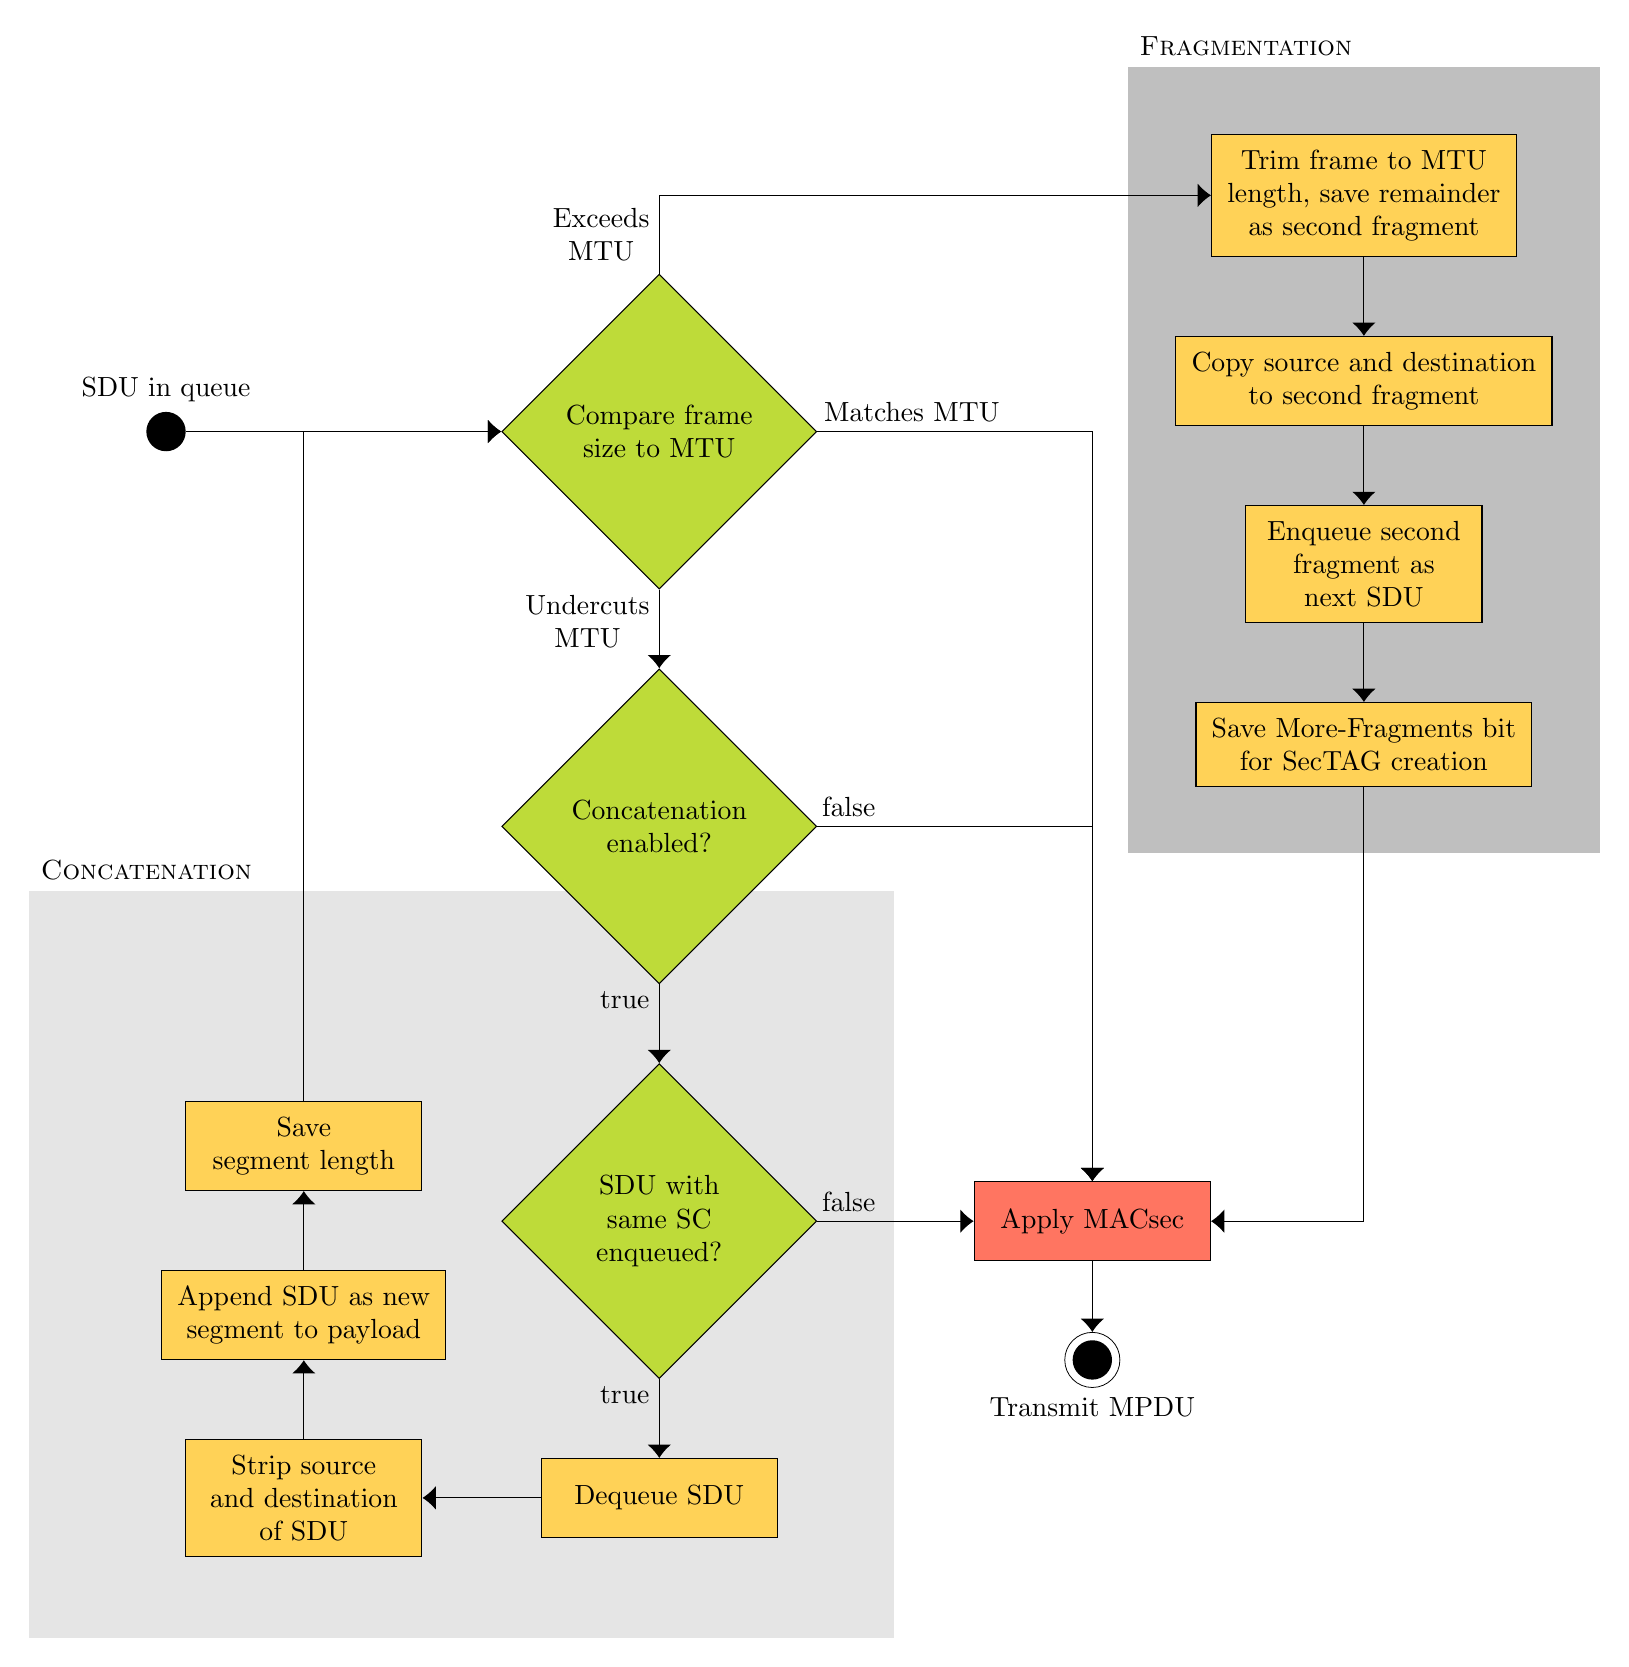
\begin{tikzpicture}
    [node distance=5.5cm,
    startstop/.style={rectangle, minimum width=3cm, minimum height=1cm,text centered, draw=black, fill=pastelred},
    decision/.style={diamond, minimum width=4cm, minimum height=4cm, text centered, draw=black, fill=pastelgreen},
    process/.style={rectangle, minimum width=3cm, minimum height=1cm, text centered, draw=black, fill=pastelorange, inner sep=.2cm}]
    \node (start) [circle,fill=black,minimum size=.5cm,label=above:SDU in queue] {};
    %\node (start) [startstop, below=1cm of begin] {SDU should be sent};
    %\draw[-{Latex[width=3mm]}] (begin) -- (start);
    \node (frame-size) [decision, right=4cm of start,align=center] {Compare frame\\size to MTU};
    \draw[-{Latex[width=3mm]}] (start) -- (frame-size);

    \node (concat-enabled) [decision, below=1cm of frame-size, align=center] {Concatenation\\ enabled?};
    \draw[-{Latex[width=3mm]}] (frame-size) -- node[anchor=east,align=center,yshift=.1cm] {Undercuts\\MTU} (concat-enabled);

    \node (sdu-queue) [decision, below=1cm of concat-enabled, align=center] {SDU with\\same SC\\enqueued?};
    \draw[-{Latex[width=3mm]}] (concat-enabled) -- node[anchor=east,yshift=.3cm]{true} (sdu-queue);

    \node (dequeue) [process, below=1cm of sdu-queue] {Dequeue SDU};
    \draw[-{Latex[width=3mm]}] (sdu-queue) -- node[anchor=east,yshift=.3cm]{true} (dequeue);
    \node (cut-source) [process, left=1.5cm of dequeue, align=center] {Strip source\\ and destination\\of SDU};
    \draw[-{Latex[width=3mm]}] (dequeue) -- (cut-source);
    \node (append) [process, above=1cm of cut-source, align=center] {Append SDU as new\\segment to payload};
    \draw[-{Latex[width=3mm]}] (cut-source) -- (append);
    \node (save-length) [process, above=1cm of append, align=center] {Save\\ segment length};
    \draw[-{Latex[width=3mm]}] (append) -- (save-length);
    \draw[-{Latex[width=3mm]}] (save-length) |- (frame-size);

    \node (split-sdu) [process, right=5cm of frame-size, align=center,yshift=3cm] {Trim frame to MTU\\length, save remainder\\as second fragment};
    \draw[-{Latex[width=3mm]}] (frame-size) |- node[anchor=east, align=center,yshift=-.5cm]{Exceeds\\MTU} (split-sdu);
    \node (copy-src) [process, below=1cm of split-sdu, align=center] {Copy source and destination\\to second fragment};
    \node (enqueue-fragment) [process, below=1cm of copy-src, align=center] {Enqueue second\\fragment as\\next SDU};
    \draw[-{Latex[width=3mm]}] (split-sdu) -- (copy-src);
    \draw[-{Latex[width=3mm]}] (copy-src) -- (enqueue-fragment);
    \node (save-mf) [process, below=1cm of enqueue-fragment, align=center] {Save More-Fragments bit\\for SecTAG creation};
    \node (end) [startstop, right of=sdu-queue] {Apply MACsec};

    \node (stop) [circle,minimum size=.5cm, line width=.01cm, fill=black, below=1cm of end] {};
    \node (stop2) at (stop) [circle,minimum size=.7cm, line width=.01cm, draw=black,label=below:Transmit MPDU] {};

    \draw[-{Latex[width=3mm]}] (frame-size) -| node[anchor=south,pos=.0,xshift=1.2cm] {Matches MTU} (end);
    \draw[-{Latex[width=3mm]}] (concat-enabled) -| node[anchor=south,pos=.0,xshift=0.4cm]{false} (end);
    \draw[-{Latex[width=3mm]}] (sdu-queue) -- node[anchor=south,pos=.0,xshift=0.4cm]{false} (end);

    \draw[-{Latex[width=3mm]}] (enqueue-fragment) -- (save-mf);
    \draw[-{Latex[width=3mm]}] (save-mf) |- (end);
    \draw[-{Latex[width=3mm]}] (end) -- (stop2);

    \begin{pgfonlayer}{bg}
      \node at (save-length) [draw,color=white,fill=gray!20,rectangle,yshift=-1.5cm,xshift=2cm,minimum width=11cm,minimum height=9.5cm,label={[xshift=-4cm,align=left]above:\textsc{Concatenation}}] {};

      \node at (copy-src) [draw,color=white,fill=gray!50,rectangle,xshift=0cm,yshift=-1cm,minimum width=6cm,minimum height=10cm,label={[xshift=-1.5cm]above:\textsc{Fragmentation}}] {};
    \end{pgfonlayer}

  \end{tikzpicture}
%\end{document}

    }
    \caption[Transmission Flowchart]{Transmission flowchart for proposed modifications}
    \label{fig:fragmentation-flowchart}
\end{figure}
\subsection{Transmission Process}

The following transmission flow is displayed as flowchart in figure~\ref{fig:fragmentation-flowchart} for a better understandability.

When a frame has to be sent using \gls{MACsec} it must be checked at the beginning whether fragmentation has to be applied.
This is the case if the size of the \gls{SDU} exceeds the maximum payload size of \gls{MACsec} regarding the \gls{MTU} of the underneath layer.
If the standard \gls{MTU} of 1500 bytes is set, the maximum payload size is 1468 bytes.

The fragmentation process must happen before applying \gls{MACsec}.
Therefore, the \gls{SDU} must be split.
The first fragment must be sent with the \acrfull{MF} bit set.
It must be ensured that the second fragment is processed next by \gls{MACsec}.

If the size of the \gls{SDU} undercuts the maximum payload size of \gls{MACsec}, concatenation must be applied if enabled.
Therefore, the queue of \gls{MACsec} has to be checked for additional \glspl{SDU} that belong to the same \acrfull{SC}.
If it contains \glspl{SDU}, they are dequeued and appended to the payload until the maximum payload size is matched or exceeded.
Source and Destination addresses of these \glspl{SDU} are cut.
It must be considered that for each additional \gls{SDU} the maximum payload is decreased by two bytes because an extension header must be added.
The last \gls{SDU} may be fragmented if otherwise the maximum payload size is exceeded.
The lengths of the additional \glspl{SDU} are saved for the creation of the \gls{SecTAG}.

When creating the \gls{SecTAG} for each additional \gls{SDU} an extension header is appended to the \gls{SecTAG}.
The extension header contains the size of the corresponding \gls{SDU}.
The $n$th extension header corresponds to the $n+1$th \gls{SDU}.
The \acrlong{E} bit is set for all but the last extension headers.

After the fragmentation and concatenation process, \gls{MACsec} is applied as usual.
\begin{figure}
    \centering
    \resizebox{\columnwidth}{!}{
      %!TEX root=../thesis.tex
%\documentclass{article}
%\usepackage{geometry}
%\usepackage{tikz}
%\usetikzlibrary{matrix,calc,shapes,positioning}
%\begin{document}
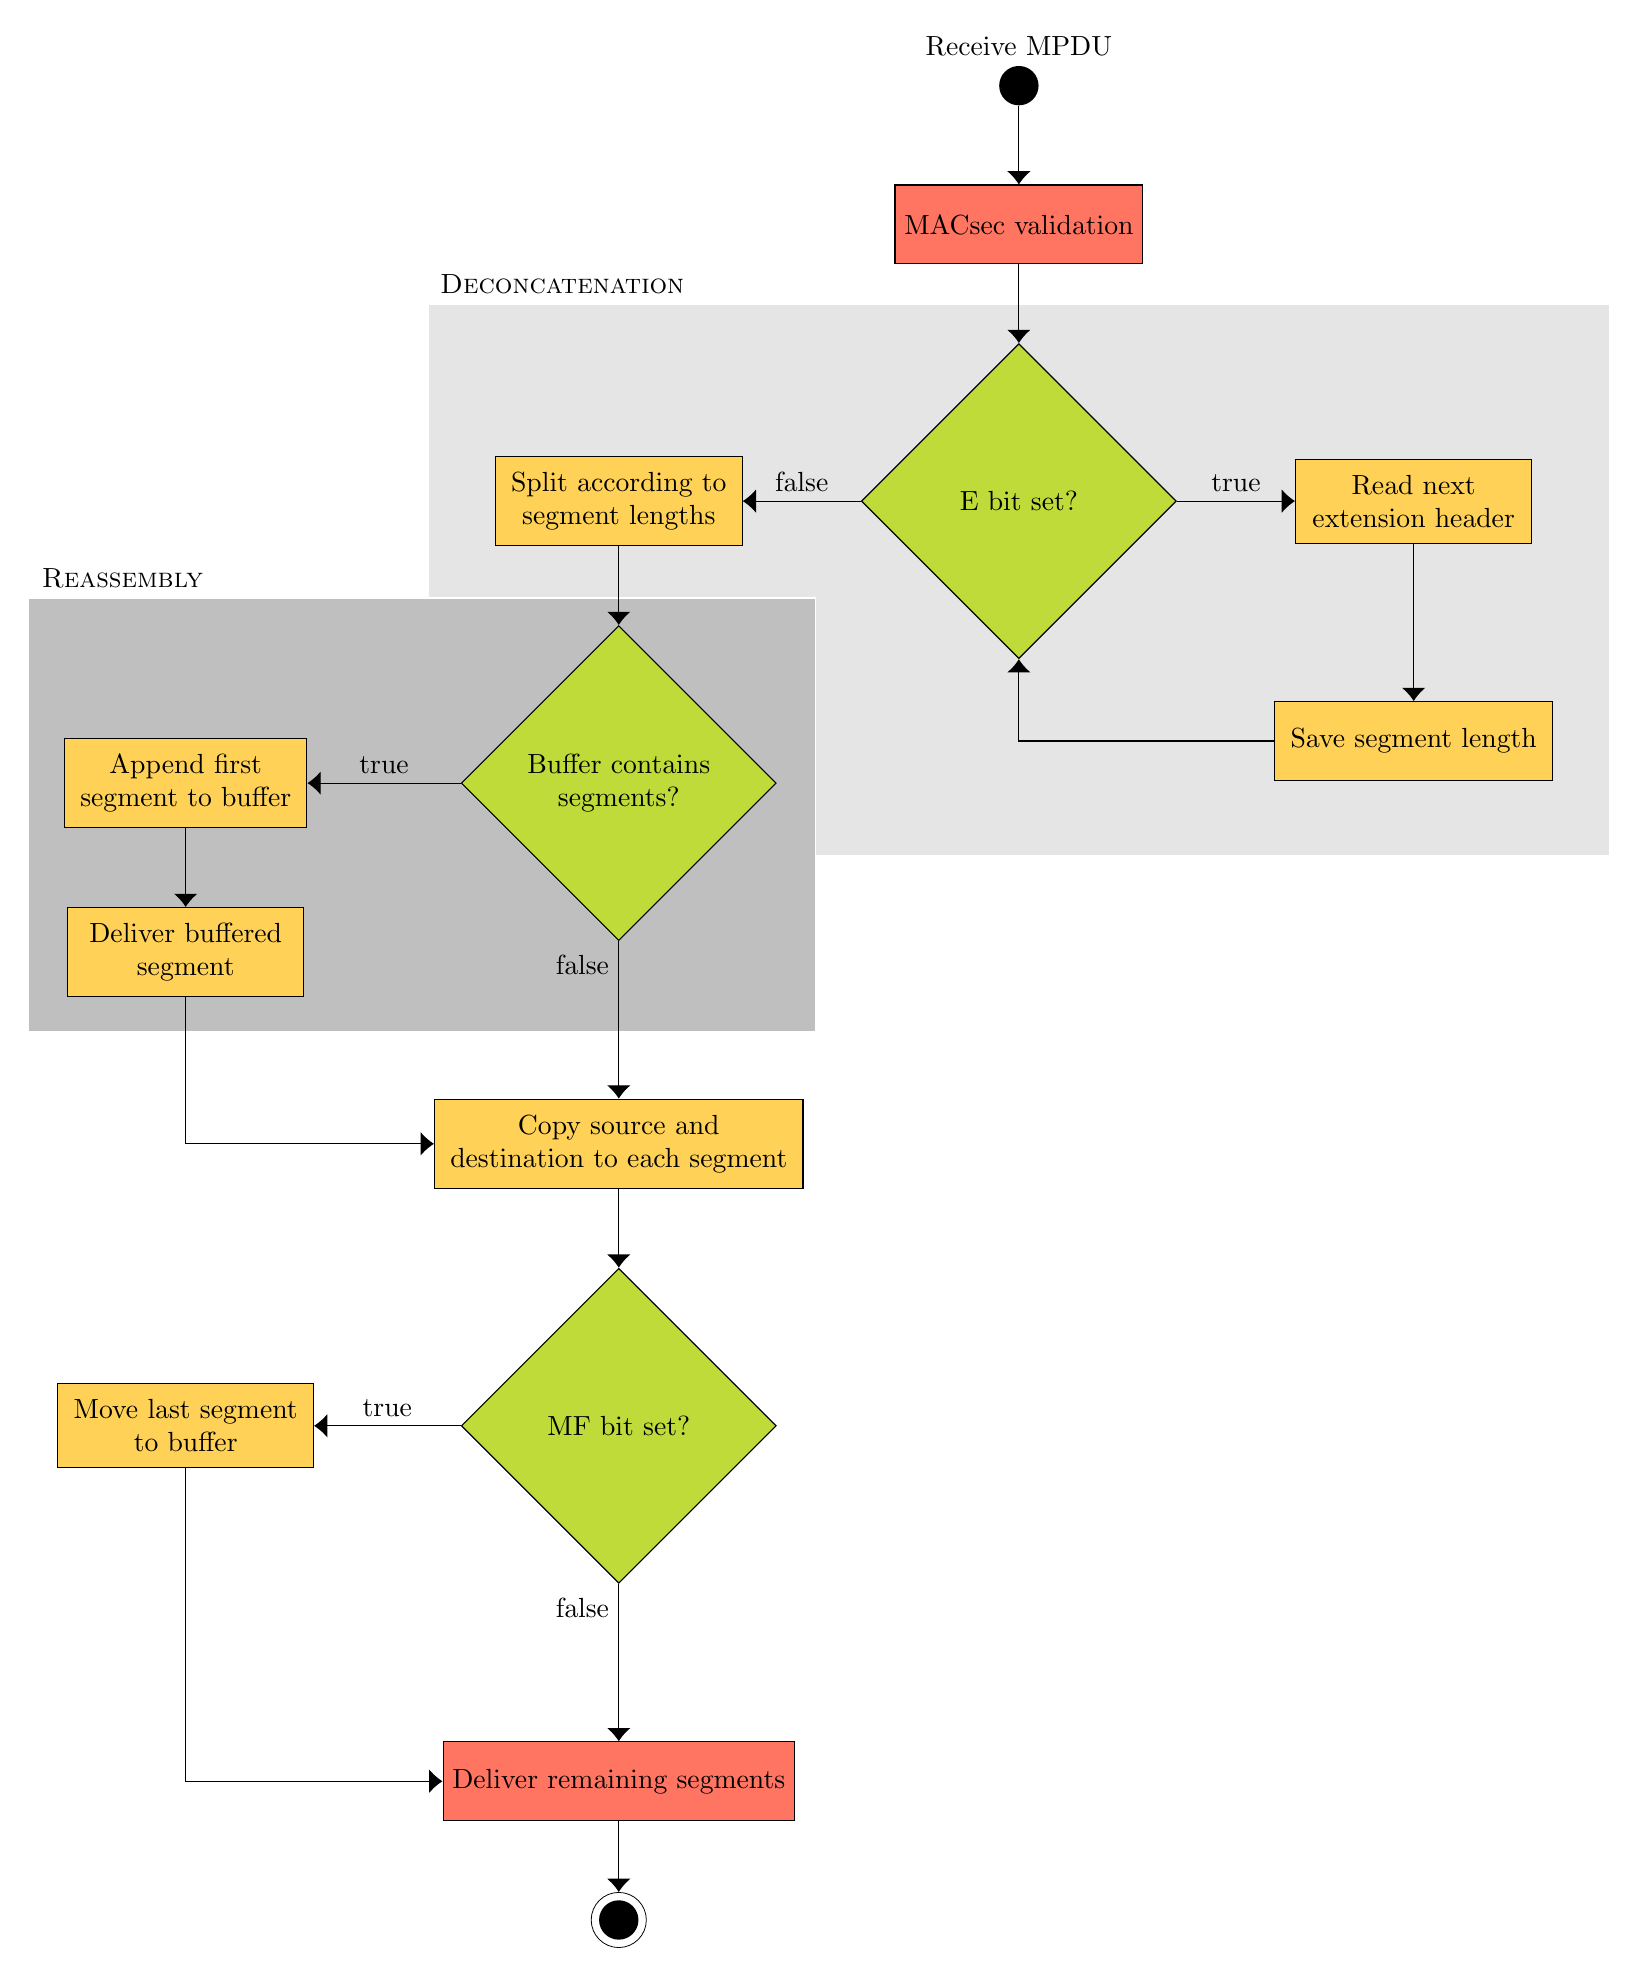
\begin{tikzpicture}
  [node distance=5.5cm,
  startstop/.style={rectangle, minimum width=3cm, minimum height=1cm,text centered, draw=black, fill=pastelred},
  decision/.style={diamond, minimum width=4cm, minimum height=4cm, text centered, draw=black, fill=pastelgreen},
  process/.style={rectangle, minimum width=3cm, minimum height=1cm, text centered, draw=black, fill=pastelorange, inner sep=.2cm}]
  \node (begin) [circle,minimum size=.5cm, line width=.01cm, fill=black,label=above:Receive MPDU] {};
  \node (macsec) [startstop, below=1cm of begin] {MACsec validation};
  \draw[-{Latex[width=3mm]}] (begin) -- (macsec);
  \node (e-bit) [decision, below=1cm of macsec] {E bit set?};
  \draw[-{Latex[width=3mm]}] (macsec) -- (e-bit);

% De-concatenate
\node (read-ext-header) [process, right=1.5cm of e-bit, align=center] {Read next\\extension header};
\draw[-{Latex[width=3mm]}] (e-bit) --node[anchor=south]{true} (read-ext-header);
\node (save-len) [process, below=2cm of read-ext-header] {Save segment length};
\draw[-{Latex[width=3mm]}] (read-ext-header) -- (save-len);
\draw[-{Latex[width=3mm]}] (save-len) -| (e-bit);
\node (split) [process, left=1.5cm of e-bit, align=center] {Split according to\\segment lengths};
\draw[-{Latex[width=3mm]}] (e-bit) --node[anchor=south]{false} (split);

% Reassembly
\node (buffer-empty) [decision, below=1cm of split, align=center] {Buffer contains\\segments?};
\draw[-{Latex[width=3mm]}] (split) -- (buffer-empty);
\node (append-to-buffer) [process, left of=buffer-empty, align=center] {Append first\\segment to buffer};
\draw[-{Latex[width=3mm]}] (buffer-empty) --node[anchor=south]{true} (append-to-buffer);
\node (deliver-buffer) [process, below=1cm of append-to-buffer,align=center] {Deliver buffered\\segment};
\draw[-{Latex[width=3mm]}] (append-to-buffer) -- (deliver-buffer);
\node (copy-src-dest) [process, below=2cm of buffer-empty,align=center] {Copy source and\\destination to each segment};
\draw[-{Latex[width=3mm]}] (deliver-buffer) |- (copy-src-dest);
\draw[-{Latex[width=3mm]}] (buffer-empty) --node[anchor=east,pos=.0,yshift=-.3cm]{false} (copy-src-dest);

% Fragmentation
\node (mf-set) [decision, below=1cm of copy-src-dest, align=center] {MF bit set?};
\node (buffer-last) [process, left of=mf-set,align=center] {Move last segment\\to buffer};
\node (deliver) [startstop, below=2cm of mf-set] {Deliver remaining segments};
\node (stop) [circle,minimum size=.5cm, line width=.01cm, fill=black, below=1cm of deliver] {};
\node (stop2) at (stop) [circle,minimum size=.7cm, line width=.01cm, draw=black] {};
\draw[-{Latex[width=3mm]}] (deliver) -- (stop2);


\draw[-{Latex[width=3mm]}] (copy-src-dest) -- (mf-set);
\draw[-{Latex[width=3mm]}] (mf-set) --node[anchor=east,pos=.0,yshift=-.3cm]{false} (deliver);
\draw[-{Latex[width=3mm]}] (mf-set) --node[anchor=south]{true} (buffer-last);
\draw[-{Latex[width=3mm]}] (buffer-last) |- (deliver);
  \begin{pgfonlayer}{bg}
    \node at (e-bit) [draw,color=white,fill=gray!20,rectangle,yshift=-1cm,minimum width=15cm,minimum height=7cm,label={[xshift=-5.8cm]above:\textsc{Deconcatenation}}] {};

    \node at (append-to-buffer) [draw,color=white,fill=gray!50,rectangle,xshift=3cm,yshift=-.4cm,minimum width=10cm,minimum height=5.5cm,label={[xshift=-3.8cm]above:\textsc{Reassembly}}] {};
  \end{pgfonlayer}
\end{tikzpicture}
%\end{document}

    }
    \caption[Receive Flowchart]{Receive flowchart for proposed modifications}
    \label{fig:receive-flowchart}
\end{figure}
\pagebreak
\subsection{Receiving Process}
The following receive flow is displayed as flowchart in figure~\ref{fig:receive-flowchart}.

When a frame is received it must be validated as specified by the original \gls{MACsec} standard.
Except to this validation is the check if both reserved bits of the \gls{SL} field are set as these are now the \gls{E} and \gls{MF} bit.

If the validation is successful, it is checked whether the \gls{E} bit is set.
If the \gls{E} bit is set, all extension headers are processed and the payload is cut into several \glspl{SDU}.
The length of each one is derived by the extension headers.
The Source- and Destination addresses are prepended to each \gls{SDU}.
If the \gls{E} bit is not set, the payload contains only one \gls{SDU}.

If the fragmentation buffer for the current \gls{SC} contains any data, the first \gls{SDU} must be prepended to this data and the whole, new \gls{SDU} must be delivered.
If the \gls{MF} bit is set, the last \gls{SDU} has to be saved into the buffer for the current \gls{SC}.

Finally, all remaining \glspl{SDU} are delivered.

\subsection{\acrlong{MPDU}}

\begin{figure}
  \centering
  \begin{bytefield}[bitwidth=0.0625\columnwidth]{8}
    \bitheader{1-8} \\
      \wordbox[lrt]{1}{Segment Length} \\
      \bitbox[lrb]{3}{ } & \colorbitbox{lightgray}{4}{} & \bitbox{1}{E}
  \end{bytefield}
  \caption[Extension header of modified \acrshort{MACsec}]{Extension header of modified \gls{MACsec}}
  \label{fig:extension-header}
\end{figure}


The modified \gls{MPDU} is displayed in figure~\ref{fig:concat-sectag}.
The first unused bit after the \acrlong{SL} field is the \gls{MF} bit.
This bit indicates whether the payload is fragmented and the next frame contains the next fragment.
The second unused bit after the \acrlong{SL} field is the \gls{E} bit.
This bit indicates whether an extension header is appended to the \gls{SecTAG}.

The extension header comprises of an 11 bit long \acrfull{SEGL} field and an \gls{E} bit.
These are seperated by 4 unused bits.
The \gls{SEGL} field contains the length of the corresponding \gls{SDU}.
The $n$th extension header corresponds to the $n + 1$th \gls{SDU}.
If the \gls{E} bit of an extension header is set, another extension header follows.
Otherwise, the payload follows.

  %!TEX root=../thesis.tex
\section{Implementation}
\label{ch:implementation}
In 2016 the \gls{MACsec} kernel driver implemented by \textsc{Sabrina Dubroca} was merged into the linux kernel\footnote{\url{https://git.kernel.org/pub/scm/linux/kernel/git/torvalds/linux.git/commit/?id=c09440f7dcb304002dfced8c0fea289eb25f2da0}}.
The design specified in the previous chapter is implemented based on the kernel version 4.15.6\footnote{\url{https://git.kernel.org/pub/scm/linux/kernel/git/stable/linux-stable-rc.git/commit/?h=v4.15.6&id=1a7aef62b47b00630e62a268d647f54ec93fb38c}}.

In~\cite{dubrocamacsec} \textsc{Dubroca} describes the implementation details of the \gls{MACsec} driver.
\gls{MACsec} is implemented as a virtual network device.
There are two important entry points regarding the proposed changes.
When a new frame is sent via the \gls{MACsec} device, the function \inlinecode{c}{macsec_start_xmit} is executed with the frame as parameter.
When a frame is received by the \gls{MACsec} device, the \inlinecode{c}{rx_handler} \inlinecode{c}{macsec_handle_frame} function is executed.

Frames in the linux kernel are represented by \inlinecode{c}{struct sk_buff}, which is an abbreviation of socket buffer.
This struct contains multiple pointers to the actual data.

The \gls{MACsec} frame header is represented by the \inlinecode{c}{struct macsec_eth_header}.
To reflect the proposed changes of the \gls{MPDU}, it now contains the \acrlong{MF} and \acrlong{E} bits as well as an arbitrary number of extension headers as shown in the implementation excerpt~\ref{lst:macsec-hdr}.

The \gls{MTU} of the \gls{MACsec} device is calculated by subtracting the size of the \gls{SecTAG} and \gls{ICV} from the \gls{MTU} of the underlaying network device.
To reflect the increased \gls{MTU}, a constant---\inlinecode{c}{#define ADDITIONAL_MTU 1468}---is introduced and added to this value.
\begin{figure}
  \lstset{language=C}
  \begin{lstlisting}
  struct macsec_eth_header {
      struct ethhdr eth;
      u8  tci_an;
      u8  short_length:6
          more_fragments:1
          extended:1;
      __be32 packet_number;
      u8 secure_channel_id[8];
  } __packed;
  \end{lstlisting}
  \caption{\acrshort{MACsec} header struct}
  \label{lst:macsec-hdr}
\end{figure}

\subsection{Fragmentation}
The fragmentation is implemented in the transmission handler function \inlinecode{c}{macsec_start_xmit}.
Therefore, the size of the socket buffer is checked.
If its current size added to the additional \gls{MACsec} size is larger than the \gls{MTU} of the underlaying device a fragment has to be created.
Therefore, a second socket buffer is allocated.
The ethernet header is copied and the payload is split up between both frames.
After that, each step is executed on both socket buffers if fragmentation occurs.
To ensure the correct order of both frames, the second socket buffer is transmitted directly after the first socket buffer.

\subsection{Reassembly}
The reassembly takes place after the \gls{MACsec} frame is validated and the \gls{SecTAG} and \gls{ICV} are stripped.
If the \acrfull{MF} bit is set, the payload, its length and the original Ethertype are saved in a double linked list as shown in~\ref{lst:frag_buff}.
As every \acrfull{SC} has its own buffer the network device is still able to receive frames of different \glspl{SC}.

\begin{figure}
  \lstset{language=C}
  \begin{lstlisting}
  struct macsec_fragmentation_buffer {
    sci_t sci;
    struct macsec_fragmentation_buffer *next;
    struct macsec_fragmentation_buffer *prev;
    unsigned char *data;
    unsigned int len;
    unsigned short proto;
  }
  \end{lstlisting}
  \caption{Fragment buffer data structure}
  \label{lst:frag_buff}
\end{figure}

When a frame arrives that does not have the \gls{MF} bit set, it is checked whether data is buffered for this \gls{SC}.
If this is the case, the data of the fragmentation buffer is prepended to the payload of the frame.
Additionally, the Ethertype is set according to the saved one.
After the buffer is cleared, the frame is delivered.

\subsection{Challenges}
While implementing the proposed modifications of \gls{MACsec}, several issues arised.
The three most significant ones are described in the following paragraphs.

\paragraph{Order of frames}
\label{par:frame-order}
The protocol relies on the correct order of frames.
As both endpoints are connected directly, it must be ensured that the network interface retains the order on transmission.
Therefore, the new \gls{MACsec} driver transmits both fragments successively to the network interface.

Each network interface has a configured algorithm which manages the queue.
This group of algorithms is named \glspl{Qdisc}~\cite{hubert2002linux}.
A simple \gls{Qdisc} is \gls{FIFO}---packets are sent in the order they arrive.
There are also \glspl{Qdisc}, which do not retain the order of frames as they arrive, but prefer some with certain properties.
One of them is FQ\_CoDel\footnote{\url{http://man7.org/linux/man-pages/man8/tc-fq_codel.8.html}}, which drops packets with a high queing delay.

The \gls{Qdisc} FQ\_CoDel has been set for the network interface on the used test system.
This led to high retransmission and error rates while using ``iperf3''.

As the virtual device should not change the configuration of the underlaying network interface, it does not set a \gls{Qdisc}.
The only solution that may seem reasonable is to print a warning to kernel log, if a \gls{Qdisc} differs from \gls{FIFO}, as this may decrease the performance of \gls{MACsec} fragmentation significantly.

\paragraph{Concatenation}
The implementation of the concatenation algorithm has several requirements, two of them are the possibility to access and manipulate the queue of the \gls{MACsec} device.
By default the \gls{MACsec} device has no queue but after configuring a \gls{Qdisc}---which is described in the previous section---it was possible to access it.
When concatenation of several \glspl{SDU} happens, it may occur that the last \gls{SDU} must additionally be fragmented.
If this happens, it must be guaranteed that the last fragment of this \gls{SDU} is sent in the next \gls{MACsec} frame.
Thus, this fragment must be the next one processed by the \gls{MACsec} device and the queue must be manipulated to achieve that.
After some investigation, it was possible to dequeue and enqueue \glspl{SDU}, but not to manipulate the order of the queue.
For time reasons, it was not possible to implement this manipulation and hence the current implementation does not support concatentation.

\paragraph{Fragmentation of TCP packets}
If the socket buffer has to be fragmented, it is split into two parts.
Therefore, the original buffer is trimmed and the remaining payload is moved to another position, where the fragment points to.

To test the implementation the command line tools \inlinecode{bash}{ping}---which sends ICMP packets---and  \inlinecode{bash}{iperf3}---which sends \gls{TCP} packets---where used.
In the beginning of each test everything worked but when \inlinecode{bash}{iperf3} was used after a varying amount of time the kernel crashed.

After many debugging attempts, the reliability of \gls{TCP} turned out to be a problem.
\gls{TCP} retransmits a packet when no acknowledge is received.
Therefore, the kernel keeps a pointer of the socket buffer, so on retransmission the frame must not be recreated.
If the socket buffer was fragmented by \gls{MACsec} the kernel expected a longer one which led to a kernel panic.

To solve this problem, the implementation now checks, whether a reference to the socket buffer is still hold by anyone.
If this is the case the socket buffer and its data is cloned, so if \gls{TCP} now retransmits a packet it is not modified.
This is recommended by the documentation\footnote{\url{https://www.fsl.cs.sunysb.edu/kernel-api/re501.html}}.

  %!TEX root=../thesis.tex
\chapter{Evaluation}
\label{ch:eva}
% Intel(R) Core(TM) i5-4590 CPU @ 3.30GHz
% Intel® Ethernet Connection I217-LM
% 16GB RAM
% CAT 5E Gigabit Ethernet

% Erst Ziele, warum? Messwerte -> Setup -> Ergebnisse -> Auswertung -> Bewertung
The problem of a decreased \gls{MTU} when using \gls{MACsec} is solved with the proposed modifications of chapter~\ref{ch:design}, which were implemented as described in section~\ref{ch:implementation}.

To assess, if these modifications lead to significant performance changes, several measurments were made.
These are compared with the solution of using jumbo frames, which is also a possibility to mitigate the problem of a lower \gls{MTU}.
This solution is considered to be optimal but not applicable in the given scenario.

As the modified driver is sending two frames instead of one considering a large frame, \acrfull{RTT} might be affected.
Furthermore, an additional \gls{MACsec} header must be sent, which might affect the bandwidth.
As a third measurement the CPU usage during the bandwidth test is recorded, to see if the fragmentation and reassembly has a significant impact on it.

For the evaluation two computers are directly connected to each other with a Cat5e network cable.
Table~\ref{tab:eva-hardware} contains the hardware specifications of both machines.
\begin{table}[h]
  \centering
  \begin{tabular}{l  r}
    Processor & Intel i5-4590 3.3GHz\\
    RAM & 16GB\\
    Network interface & Fast Ethernet \& Gigabit Ethernet\\
    Operating System & Arch Linux\footnotemark with linux kernel 4.15.7\\
  \end{tabular}
  \caption{Specifications of the machines used for the evaluation}
  \label{tab:eva-hardware}
\end{table}
\footnotetext{\url{https://www.archlinux.org/}}

\section{Experiment}
Evaluated is the \gls{RTT} and bandwidth.
For the measurement of the \gls{RTT} the command line tool ``ping'' is used.
The bandwidth is measured with ``iperf3''\footnote{\url{http://software.es.net/iperf/}}.

The test cases are:
\begin{itemize}
  \item Ethernet with \gls{MTU} of 1468 bytes, 1500 bytes and 2936 bytes
  \item \gls{MACsec} with \gls{MTU} of 1468 bytes, 1500 bytes and 2936 bytes by enabling Jumbo Frames
  \item Modified \gls{MACsec} with \gls{MTU} of 1468 bytes, 1500 bytes and 2936 bytes
\end{itemize}

The \gls{MTU} of 1468 bytes is chosen because it is the standard \gls{MACsec} \gls{MTU}.
With this \gls{MTU} the modified \gls{MACsec} does not do any fragmentation.
The \gls{MTU} of 1500 bytes is chosen because it is the standard ethernet \gls{MTU}.
And with an \gls{MTU} of 2936 bytes the modified \gls{MACsec} version sends two full frames, instead of one full and one small frame as in the setting with an \gls{MTU} of 1500 bytes.

The measurement is automated with a shell script, which runs on one of both machines.
In the following, this machine is referred to as sender and the other one as receipient.

In the beginning, the sender sets the configuration according to the current test case.
After that, it configures the receipient and starts an iperf3 server via ssh.
A single bandwidth measurement performs a 10~second long iperf3 test, which builds up a \gls{TCP} connection and measures the average bandwidth.
This test is repeated 1000 times for each test case, except the Ethernet case with a \gls{MTU} of 2936 bytes where it is repeated 100 times.
The ethernet test case is interesting for comparability but plays a minor role for the assessment of the \gls{MACsec} modifications.
For the \gls{RTT} measurment an adaptive ping is started, which sends and receives 50000 \gls{ICMP} messages.
Usually, ping sends one echo request every second but with the adaptive ping it sends the next request as soon as the last was acknowledged.

\section{Measurements}
\subsection{\acrlong{RTT}}
\begin{figure}
    \centering
    \def\svgwidth{\columnwidth}
    \input{./figures/rtt-boxplot.pdf_tex}
    \caption[\acrlong{RTT} experiment]{\gls{RTT} measurements for the different test cases.\\$n=50000$}
    \label{fig:rtt-test}
\end{figure}

The results of the \gls{RTT} are displayed in figure~\ref{fig:rtt-test} and table~\ref{tab:rtt-data}.
It is noticeable that two test cases which used jumbo frames---Ethernet and \gls{MACsec} with an \gls{MTU} of 2936 bytes---have a significant higher \gls{RTT} (0.44ms to 0.52ms) and higher variance, compared with the remaining test cases (0.14ms to 0.17ms).

The reasons for this are not further researched in this thesis but there are several publications which detect a high latency when using jumbo frames~\cite{chelseajumbo}.

To make the results of the other test cases more visible, both described cases are removed in figure~\ref{fig:rtt-test-zoom}.
\begin{figure}
    \centering
    \def\svgwidth{\columnwidth}
    \input{./figures/rtt-boxplot-zoom.pdf_tex}
    \caption[\acrlong{RTT} experiment (clipped)]{Clipped \gls{RTT} measurements for the different test cases, full results visible in figure~\ref{fig:rtt-test}.\\$n=50000$}
    \label{fig:rtt-test-zoom}
\end{figure}

The \gls{RTT} of Ethernet with an \gls{MTU} of 1468 bytes (0.139ms) respectively 1500 bytes (0.14ms) is lower than the \gls{RTT} of the test cases where \gls{MACsec} is used.
It can be assumed that this is a result of the cryptographic operations when using \gls{MACsec}.

It is noticeable that the modified \gls{MACsec} (0.155ms) has a similar \gls{RTT} as the unmodified \gls{MACsec} (0.154ms) with a frame size of 1468 bytes.
Here, no fragmentation happens.
When the modified \gls{MACsec} does fragmentation with a frame size of 1500 bytes, the \gls{RTT} increases to 0.166ms.
Compared to \gls{MACsec} with jumbo frames and a \gls{MTU} of 1500 bytes (0.155ms) this is an increase of 7.1\%.
It is assumed that this is the result of having to send two frames instead of one.
The modified \gls{MACsec} with an \gls{MTU} of 2936 bytes has an increased \gls{RTT} (0.174ms), which might be the result of a bigger frame which has to be sent.
But compared to \gls{MACsec} with jumbo frames and an \gls{MTU} of 2936 bytes it is significant faster.

\subsection{Bandwidth}
\label{sec:bandwidth-eva}
\begin{figure}
    \centering
    \def\svgwidth{\columnwidth}
    \input{./figures/bandwidth-bar.pdf_tex}
    \caption[Bandwidth experiment bar chart]{Bandwidth measurements for the different test cases.\\$n=1000$, except for Ethernet with MTU 2936 $n=100$}
    \label{fig:bandwidth-test}
\end{figure}
The results of the bandwidth test are shown in figure~\ref{fig:bandwidth-test} and table~\ref{tab:bandwidth-data}.

The data shows that, independent of the test case, the variance is small.
All test cases where no \gls{MACsec} is used reach a higher bandwidth compared with the other test cases which had the same \gls{MTU}.
This decrease when using \gls{MACsec} might be the result of the additional 32 bytes long header, which has to be sent in each frame.

\gls{MACsec} (907.4 Mbit/s) and the modified \gls{MACsec} (907.38 Mbit/s) reach a similar bandwidth when using a frame size of 1468 bytes.
When the modified \gls{MACsec} does fragmentation, the bandwidth decreases compared to \gls{MACsec} with the same \gls{MTU} of 1500 bytes respectively 2936 bytes.
In the fragmentation cases a second Ethernet and \gls{MACsec} header have to be sent which lead to this decrease.
The modified \gls{MACsec} reaches 95\% respectively 97\% of the bandwidth that \gls{MACsec} with the same \gls{MTU} creates.

\subsection{CPU Usage}
The results of the CPU usage during the bandwidth test are shown in figure~\ref{fig:cpu-test} and table~\ref{tab:cpu-data}.
As the data is generated during the bandwidth test, the CPU usage also depends on the size of this data.

During the tests without \gls{MACsec}, the CPU usage is significantly higher (5.55\% to 5.16\%) than during the tests where \gls{MACsec} is applied (0.96\% to 2.29\%).
Furthermore, it is noticeable that the CPU usage during the tests with the modified \gls{MACsec} is in the same order of magnitude as during the use of \gls{MACsec}.

There is at least no obvious reason, why during the tests without the usage of \gls{MACsec} the CPU was used significantly more.
These were the cases, where more data for the bandwidth test was generated due to a better performance as evaluated in section~\ref{sec:bandwidth-eva}.
For investigation of this reason, a normalization of the CPU usage result was made, which is displayed in figure~\ref{fig:cpu-test-norm}.
But even here the results are significantly worse.
The results of the CPU usage measurement need more investigation.

\begin{figure}
    \centering
    \def\svgwidth{\columnwidth}
    \input{./figures/cpu-usage-boxplot.pdf_tex}
    \caption[CPU Usage experiment]{CPU usage during the different test cases regarding the bandwidth test.\\$n=1000$, except for Ethernet with MTU 2936 $n=100$}
    \label{fig:cpu-test}
\end{figure}
\begin{figure}
    \centering
    \def\svgwidth{\columnwidth}
    \input{./figures/cpu-bandwidth-boxplot.pdf_tex}
    \caption[CPU Usage normalized to sent megabytes]{Sent megabytes divided by CPU usage in percent during bandwidth test.\\$n=1000$, except for Ethernet with MTU 2936 $n=100$}
    \label{fig:cpu-test-norm}
\end{figure}

\section{Security Evaluation}
This thesis assumes that \gls{MACsec} is secure.
It provides integrity, confidentiality, data origin authenticity, and protection against replay attacks.

The proposed modifications alter the \gls{SecTAG}.
Two reserved bits are replaced by the \acrlong{MF} and \acrlong{E} bit.
Furthermore, additional extension headers may be appended to the \gls{SecTAG}.

These modifications---which are explained in further detail in chapter~\ref{ch:proposal}---are evaluated regarding security in the following paragraphs.

\subsection{Confidentiality}
\gls{MACsec} provides confidentiality by encrypting the secure payload.
This does not include the \gls{SecTAG}.

If fragmentation is applied, the \gls{SDU} is split and each part is the secure payload of one \gls{MPDU}.
If concatenation is applied, several \glspl{SDU} build the secure payload of one \gls{MPDU}.
As the secure payload is constructed before \gls{MACsec} is applied, it still provides the same confidentiality regarding the encryption of the transmitted data.
The encryption process as well as the used algorithms or keys are not modified.

The \gls{SecTAG} is extended with information of whether a fragment follows and the length of each concatenated \gls{SDU}.
The number and corresponding length of transmitted \glspl{SDU} is obtainable for an attacker, when the unmodified \gls{MACsec} is used.
Hence, no additional information is disclosed.

Therefore, confidentiality is not weakened by the proposed modifications.

\subsection{Integrity}
\gls{MACsec} provides integrity by building a message authentication code named \gls{ICV}.
The \gls{ICV} includes the source and destination adresses, the \gls{SecTAG} and the secure payload.

Fragmented as well as concatenated \glspl{SDU} are always contained in the secure payload of an \gls{MPDU} and, therefore, integrity protected by the \gls{ICV}.
The modifications of the \gls{SecTAG} are also protected by the \gls{ICV}.
The process defined in chapter~\ref{ch:proposal} specifies that on transmit the modifications and the secure payload are built before calculating the \gls{ICV}.
Furthermore, on receive the \gls{ICV} is verified before the data is processed.
Thus, an outside attacker has no possibility to modify data undetectable.
This is visible in the flowcharts describing the transmission (figure~\ref{fig:fragmentation-flowchart}) and receive (figure~\ref{fig:receive-flowchart}) process.

Therefore, the integrity is not weakened by the proposed modifications.
The data origin authenticity is guaranteed by integrity and authentication through the \acrlong{KaY}.
As integrity is not weakened and the \acrlong{KaY} is not part of \gls{MACsec} standard data origin authenticity is still ensured.

\subsection{Availability}
The proposed modifications of \gls{MACsec} specify that received data is verified by \gls{MACsec} before the process of reassembly and deconcatenation occurs.
Therefore, outside attackers cannot exploit the introduced behavior, as it is assumed that \gls{MACsec} is secure.
On transmission and receive, the proposed modifications perform similar to \gls{MACsec} as shown in the previous sections.
Inside attackers which participate legitimately in the communication can exploit the introduced behavior regarding availability, for example by sending frames which have the \gls{MF} bit set.
This leads to a reassembly of not associated fragments and therefore illegable data is delivered.
But as \gls{MACsec} does not prevent insider attacks, this is not considered.

Therefore, the availability regarding outside attackers is not weakened by the proposed modifications.

\subsection{Replay protection}
\gls{MACsec} provides replay protection by using incrementing packet numbers.
Packets with a number which was already received are dropped\footnote{The exact behavior is configurable}.
This behavior is not changed by the modifications, the check of the packet number is done before the modifications are applied.
Furthermore, the field containing and the build of the packet number is not changed.

Therefore, the replay protection of \gls{MACsec} is not weakened by the proposed modifications.
\pagebreak
\section{Results}
The results of the performance evaluation and security evaluation are satisfying.

The \gls{RTT} results are as expected if fragmentation is applied the \gls{RTT} just slightly increases.
Additionally, the results of the bandwidth test shows that the modified \gls{MACsec} still reaches 95\% of the results of \gls{MACsec} with jumbo frames.
The measurements of the CPU usage are not completely comprehensible but the results of using modified \gls{MACsec} are in the same order of magnitude as unmodified \gls{MACsec}.
The security evaluation shows that the proposed modifications maintain the security level of \gls{MACsec}.

The proposed modifications appear to successfully solve the given problem without decreasing the performance significantly, as demonstrated by the prior evaluation.
A working implementation as a linux kernel module is provided.
This outcome leads to the conclusion that functionality of the proposed solution is given.

  %!TEX root=../thesis.tex
\chapter{Conclusion}
The goal of this thesis was to develop a transparent fragmentation solution while using \gls{MACsec} to mitigate the problems of a decreased \gls{MTU}.
It is required to not mitigate the problem by the use of jumbo frames or fragmentation in upper layers.
Three established fragmentation processes in computer networks were presented.
Two general approaches for the given problem were deduced and discussed.
The approach of fragmenting \glspl{MPDU} turned out to be vulnerable, so the approach of fragmenting \glspl{SDU} was choosen.
To optimize this solution a concatenation scheme was developed.
The fragmentation solution was implemented in C for the linux kernel.
The concatenation scheme was not implemented.
The implemented algorithm in \gls{MACsec} was then evaluated regarding performance and security.
For evaluation of performance the implementation was deployed to two physical machines.
The results of this evaluation were compared to the solution of using jumbo frames, which is considered as an optimal solution.
Here, the proposed solution appeared to be successful, as the performance results were just slightly below the results of the optimum.
Furthermore, the security evaluation showed that the proposed solution is secure.

The solution of fragmenting \glspl{SDU} solves the problem of a decreased \gls{MTU} when using \gls{MACsec}.
It performs well---as the evaluation showed---and maintains the security which is established by \gls{MACsec}.
The developed improvement of a concatenation process appeared to be an optimization, which could be implemented and evaluated by future work.
Moreover, the field of other improvements and optimizations for \gls{MACsec} can be researched.
The behavior when using Jumbo Frames seems to be an interesting topic which can be investigated, as the evaluation detected some notable deviations from expected behavior.

  %!TEX root=../thesis.tex
\chapter{Appendix}
\section{Measured Data}
The following tables contain the measured data of the experiment described in chapter~\ref{ch:eva}.
\begin{table}[h]
  \centering
  \begin{tabular}{llrrr}
    \toprule
    & & \multicolumn{3}{c}{Percentile in ms} \\ \cmidrule(r){3-5}
    Test Case & MTU in & 25th & 50th & 75th\\
    \midrule
    Ethernet & 1468 &0.137 &0.139 & 0.140 \\
    & 1500 & 0.138 & 0.140 & 0.146 \\
    & 2936 & 0.440 & 0.520 & 0.579 \\
    %\midrule
    MACsec & 1468 &0.146 & 0.154 & 0.159 \\
     & 1500 & 0.146 & 0.155 & 0.160 \\
     & 2936 & 0.279 & 0.444 & 0.470 \\
     %\midrule
    Modified MACsec & 1468 & 0.146 & 0.155 & 0.160 \\
     & 1500 & 0.161 & 0.166 & 0.169 \\
     & 2936 & 0.161 & 0.174 & 0.178 \\
     \bottomrule
  \end{tabular}
  \caption{\acrlong{RTT} measurement}
  \label{tab:rtt-data}
\end{table}
\begin{table}[h]
  \centering
  \begin{tabular}{llrrr}
    \toprule
    & & \multicolumn{3}{c}{Percentile in Mbit/s} \\ \cmidrule(r){3-5}
    Test Case & MTU in& 25th & 50th & 75th\\
    \midrule
   Ethernet & 1468 & 929.23 & 929.30 & 929.40\\
& 1500 & 930.60 & 930.69 & 930.75\\
& 2936 & 962.46 & 962.48 & 962.49\\
MACsec & 1468 & 907.40 & 907.51 & 907.64\\
& 1500 & 908.94 & 909.03 & 909.15\\
& 2936 & 950.01 & 950.05 & 950.26\\
Modified MACsec & 1468 & 907.38 & 907.51 & 907.64\\
& 1500 & 863.95 & 864.19 & 864.41\\
& 2936 & 924.75 & 924.90 & 925.06\\
\bottomrule
  \end{tabular}
  \caption{Bandwidth measurement}
  \label{tab:bandwidth-data}
\end{table}
\begin{table}[h]
  \centering
  \begin{tabular}{llrrr}
    \toprule
    & & \multicolumn{3}{c}{Percentile in \%} \\ \cmidrule(r){3-5}
    Test Case & MTU in byte & 25th & 50th & 75th\\
    \midrule
   Ethernet & 1468 & 4.55& 4.70& 4.81\\
    & 1500& 4.59& 4.74& 4.84\\
    & 2936& 4.80& 5.02& 5.16\\
    MACsec & 1468& 0.97& 1.04& 1.11\\
    & 1500& 1.87& 1.93& 2.00\\
    & 2936& 2.07& 2.24& 2.29\\
    Modified MACsec & 1468& 0.96& 1.03& 1.10\\
    & 1500& 1.64& 1.70& 1.77\\
    & 2936& 1.04& 1.06& 1.08\\
    \bottomrule
  \end{tabular}
  \caption[CPU Usage during bandwidth test]{CPU usage in percent on the sender machine during the bandwidth test}
  \label{tab:cpu-data}
\end{table}


\printglossaries

  \clearpage
  %\bibliographystyle{IEEEtran}
  %\bibliography{references}

\printbibliography[heading=bibintoc]
\end{document}
